% -*- coding: utf-8 -*-

\chapter{Estado del arte}
\label{chap:antecedents}
\drop{E}{n} el siguiente capítulo se realiza una presentación de los conceptos
y tecnologías que han sido utilizadas para la elaboración del proyecto y se
hace un repaso de algunos de los trabajos y aplicaciones reales que han servido 
de inspiración para el diseño final del sistema.

%\section{Estado del arte}
%A continuación, se citan los principales elementos que constituyen la base
%teórica sobre la que se sustenta el resto del escrito.

  \section{La tecnología \acs{RFID}}
\acs{RFID} son las siglas de \emph{Radio Frequency IDentification} (en
castellano, \emph{\textbf{identificación por radiofrecuencia}}). Se trata de un
sistema de almacenamiento y recuperación de datos remoto que utiliza las ondas
de radio para transmitir la identidad (única) de un objeto.

El modo de funcionamiento de los sistemas \acs{RFID} es simple. Una
\textbf{etiqueta \acs{RFID}} (o transponedor) que contiene datos genera una
señal de radiofrecuencia con dichos datos. Esta señal es captada por un
\textbf{lector \acs{RFID}} y este la transforma a una señal digital entendible
por una aplicación específica que utilice \acs{RFID} (figura
\ref{fig:rfidSystem}).

\begin{figure}[!h]
  \begin{center}
    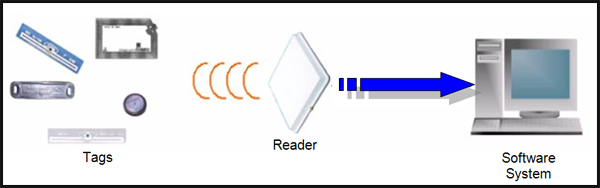
\includegraphics[width=0.8\textwidth]{rfidSystem.png}
    \caption{Esquema básico de un sistema \acs{RFID}.}
    \label{fig:rfidSystem}
  \end{center}
\end{figure}

    \subsection{Historia}
  El origen del \acs{RFID} está relacionado con la II Guerra Mundial. Los
  radares de la época eran capaces de detectar y medir la presencia de objetos
  dentro de un rango de actuación, pero no eran capaces de identificar qué
  clase de objetos eran identificados.

  Durante la década de los 50 y los 60, científicos de los países más
  avanzados, trabajaron para explicar cómo podrían identificar objetos
  remotamente. Fruto de estos estudios se inventaron los primeros sistemas
  antirrobo que funcionaban con ondas de radio. El objeto en cuestión tenía 
  una etiqueta con un único bit que decía si el artículo se había pagado o no.
  Cuando el objeto había sido pagado, se modificaba dicho bit, para que los 
  sensores de la salida no accionaran la alarma.

  Las primeras patentes fueron solicitadas en Estados Unidos en 1973. Mario W.
  Cardullo presentó una etiqueta \acs{RFID} activa que portaba una memoria
  rescribible. Y ese mismo año, Charles Walton recibió la patente para un
  sistema \ac{RFID} pasivo, consistente en una tarjeta con un transponedor que
  comunicaba una señal a un lector situado en una puerta. Si la tarjeta era
  validada por el lector, se desbloqueaba la cerradura de la puerta.

  A partir de ese año, la tecnología \acs{RFID} empezó a utilizarse por ejemplo,
  en sistemas de apertura de puertas automáticas en centrales nucleares o en
  sistemas para controlar el ganado que había sido vacunado y el que no.

  En la década de los 90, el desarrollo de nuevos materiales permitió
  reducir drásticamente el precio de las etiquetas. Este hecho favoreció
  que se potenciara el número de aplicaciones que utilizan esta tecnología.
  Es por ello que organismos internacionales empezaran a poner sus esfuerzos en
  desarrollar estándares en el uso de este tipo de etiquetas.

    \subsection{Etiquetas \acs{RFID}. Arquitectura y funcionamiento}
  Las etiquetas \acs{RFID} son dispositivos pequeños, similares a una pegatina,
  que pueden incorporarse a un objeto, un animal o una persona. 
  
  Todas las etiquetas \acs{RFID} tienen en común los siguientes elementos
  (figura \ref{fig:rfidComponents}):

  \begin{figure}[!h]
    \begin{center}
      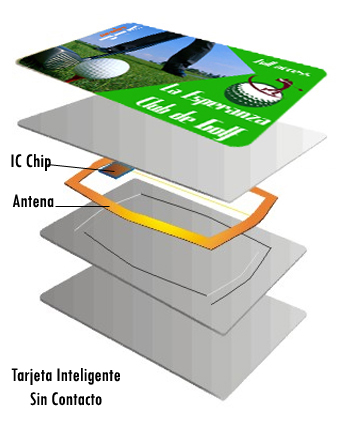
\includegraphics[width=0.4\textwidth]{rfidComponents.png}
      \caption{Componentes de una tarjeta \acs{RFID}.}
      \label{fig:rfidComponents}
    \end{center}
  \end{figure}

  \begin{itemize}
    \item \textbf{Antena}. Se encarga de recibir las señales emitidas por el
  lector y de enviar la respuesta ante dichas señales.
    \item \textbf{Chip}. Contiene la lógica de operación de la etiqueta y un
  número de identificación único.
    \item \textbf{Memoria}. Está compuesta por una parte de sólo lectura,
  que contiene las instrucciones básicas para el funcionamiento de la etiqueta;
  y por una parte de lectura y escritura, que almacena los datos escritos
  durante una comunicación con el lector.
  \end{itemize}
  
  Por otro lado, las etiquetas \ac{RFID} pueden ser de tres tipos:
  \begin{itemize}
    \item \textbf{Pasivas}. No poseen ninguna fuente autónoma de energía. La
  señal del lector es la que le induce una pequeña cantidad energía suficiente 
  como para generar y transmitir la respuesta. Tienen una fiabilidad y una
  capacidad de almacenamiento muy limitadas (unos pocos KBytes) y su campo de
  cobertura es también muy reducido (hasta 3 metros). Aún así, son las más
  utilizadas debido a su bajo coste.
   \item \textbf{Activas}. Poseen su propia fuente autónoma de energía y la
  utilizan para dar corriente a sus circuitos integrados y para propagar su
  señal al lector. Esto implica que las comunicaciones son más fiables (tienen
  menos errores), pueden transmitir señales más potentes y a mayor distancia
  (hasta 500m) y tienen más capacidad de almacenamiento. Por otro lado, tienen
  un mayor coste por chip y son de mayor tamaño que las etiquetas pasivas. La
  vida útil de sus baterías puede llegar hasta los 10 años.
    \item \textbf{Semipasivas}. Al igual que las etiquetas activas, las
  semipasivas también disponen de una fuente autónoma de energía. Sin embargo,
  estas utilizan la energía principalmente para alimentar el chip, no para
  transmitir la señal. Tienen una fiabilidad comparable a la de las etiquetas
  activas aunque superan su vida útil. Por otro lado, tienen un rango
  operativo comparable a las etiquetas pasivas aunque su respuesta es más
  rápida.
  \end{itemize}

    \subsection{Lectores RFID. Funcionamiento}
  Los lectores \acs{RFID} son los encargados de leer o re-escribir la
  información almacenada en las etiquetas.
  El funcionamiento es sencillo. La antena del lector crea un campo magnético
  y cuando este campo entra en contacto con una etiqueta, se produce la
  reacción de esta última, enviando al lector la información contenida.
  El lector decocifica los datos obtenidos y los manda a una tercera entidad 
  para que los interprete (figura \ref{fig:rfidSchema}).

  \begin{figure}[!h]
    \begin{center}
      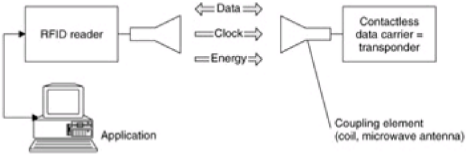
\includegraphics[width=0.8\textwidth]{rfidSchema.png}
      \caption{El lector y la etiqueta son los principales componentes de todo
sistema \acs{RFID}.}
      \label{fig:rfidSchema}
    \end{center}
  \end{figure}

  Según el número de bobinas que poseen, existen dos tipos de lectores:
  \begin{itemize}
  \item \textbf{Bobina simple}. La misma bobina crea el campo magnético y
  transmite los datos. Son más simples y baratas que las dobles y tienen
  un alcance muy limitado.
  \item \textbf{Bobina doble}. Una de las bobinas se encarga de crear el
  campo magnético y la otra de transmitir los datos. Son caras pero tienen
  mayores prestaciones que las bobinas simples.
  \end{itemize}
  
  En cuanto a la portabilidad, también existen dos tipos de lectores:
  \begin{itemize}
  \item \textbf{Lectores móviles}. Son lectores autónomos que pueden 
  transportarse a cualquier lugar y que pueden utilizarse con varios fines. Se
  comunican con otros dispositivos a través de conexiones inalámbricas.
  \item \textbf{Lectores fijos}. Son lectores ubicados en un punto fijo y 
  dedicados a un único fin. Tienen mayor rango de actuación que los lectores
  móviles y suelen utilizarse en sistemas de detección y seguimiento de
  personas y animales.
  \end{itemize}

%    \subsection{La tecnología \emph{MIFARE}}
%  \emph{MIFARE} es el estándar de la industria para interfaces de
%  tarjetas inteligentes sin contacto y lectores que operan a 13.56MHz.
%  Funcionan de acuerdo con el estándar \acs{ISO} 14443~\cite{bib:mifare}.
  
%  El alcance típico de lectura/escritura de etiquetas \emph{MIFARE} sin
%  contacto oscila entre los 2 y los 10 cm; y la capacidad más habitual está
%  entre los 1 y los 4KB de memoria \acs{EEPROM}.

%  Para que los datos sean leídos o escritos es necesaria una autentificación 
%  mútua entre el lector y la etiqueta, ya que el acceso a los mismos está 
%  protegidos por una clave de 48 bits. La transmisión de datos por
%  radiofrecuencia viaja encriptada.

%  En la actualidad \emph{MIFARE} es una marca registrada de \emph{NXP
%  Semiconductors} (empresa fundada por \emph{Philips}). Ha vendido más de 5 mil
%  millones de tarjetas y etiquetas inteligentes y más de 50 millones de
%  componentes de lectores. Ha sido seleccionada para la mayoría
%  de proyectos importantes con tarjetas inteligentes sin contacto en todo el
%  mundo y su cartera de productos incluye soluciones perfectas para la
%  recaudación automática de tarifas, tarjetas de fidelización, cobro en 
%  carreteras de peaje o gestión de acceso a edificios~\cite{bib:urlMifare} 
%  (figura \ref{fig:mifareFamily}).

%  \begin{figure}[!h]
%    \begin{center}
%      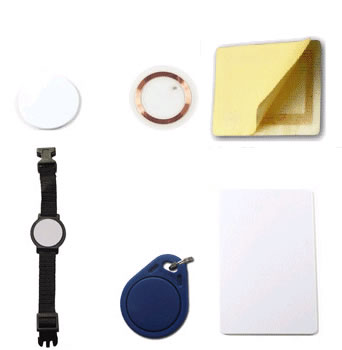
\includegraphics[width=0.5\textwidth]{mifareFamily.png}
%      \caption{Ejemplos de etiquetas MIFARE.}
%      \label{fig:mifareFamily}
%    \end{center}
%  \end{figure}

  \section{La tecnología \acs{NFC}}
\acs{NFC} son las siglas en inglés de \emph{Near Field Communication}
(Comunicación de Campo Cercano). Se trata de una tecnología inalámbrica de
corto alcance y alta frecuencia que permite el intercambio de información
entre dos dispositivos próximos entre sí.

\acs{NFC} se basa en la tecnología \acs{RFID}, que opera a 13,56MHz y tiene
una distancia de funcionamiento típica de 4 cm. Es compatible con tarjetas
inteligentes sin contacto \emph{Mifare} y \emph{FeliCa} y tiene una tasa de
intercambio de datos de hasta 424 Kb/s.

Los estándares de \acs{NFC} están basados en la \acs{ISO} 14443 e incluyen
la \acs{ISO}/\acs{IEC} 18092 y otros estándares definidos específicamente por
el \emph{NFC Forum}\footnote{Organismo formado en 2004 por los creadores de
\acs{NFC} (\emph{Nokia}, \emph{Philips} y \emph{Sony}) y que busca promover
el uso de esta tecnología. Para ello, crea especificaciones de desarrollo,
para asegurar la interoperabilidad entre dispositivos y servicios, y trata
de educar al mercado acerca de la tecnología \acs{NFC}. Actualmente, el foro
cuenta con más de 160 miembros, incluyendo fabricantes, desarrolladores de
aplicaciones, instituciones de servicios financieros, etc.~\cite{bib:nfcForum}}.

Según el propio \emph{NFC Forum}~\cite{bib:nfcForum}:

\emph{``Una tecnología de conectividad basada en estándares como \acs{NFC},
armoniza las diversas tecnologías actuales sin contacto, lo que permite
generar soluciones actuales y futuras en áreas tales como:
\begin{itemize}
\item Control de acceso.
\item Electrónica de consumo.
\item Salud.
\item Recogida e intercambio de información
\item Sistemas de fidelización y cupones.
\item Pagos.
\item Transporte.
\end{itemize}
''}.

%Una de las principales ventajas de la tecnología \acs{NFC} en los
%dispositivos móviles es que pueden ser utilizados como un dispositivo de
%almacenamiento de información, como una unidad de cómputo y como un lector
%\acs{NFC}. Esto les permite, por ejemplo, leer los datos de una etiqueta para 
%después utilizarlos como entrada en un proceso que trabaje con información 
%previamente almacenada, como ocurre en los pagos mediante \acs{NFC}.

%Otras ventajas importantes de \acs{NFC} son~\cite{bib:currentBenefits}:
%\begin{itemize}
%\item La tecnología es compatible con las estructuras existentes de \acs{RFID}.
%Es decir, etiquetas \acs{RFID} y tarjetas inteligentes sin contacto.
%\item Es fácil de usar, ya que los usuarios no necesitan tener ningún
%conocimiento sobre la tecnología. Todo lo que el usuario tiene que hacer es
%iniciar la comunicación mediante la unión o contacto de dos dispositivos.
%\item El alcance de transmisión es tan corto que, cuando el usuario separa los
%dispositivos, la comunicación se corta. Esto hace que la seguridad sea
%inherente. Si no hay ningún otro dispositivo cerca, no habrá más
%comunicaciones.
%\end{itemize}

  \subsection{Funcionamiento}
Como se comentó anteriormente, tecnología \acs{NFC} está basada en las
tecnologías de tarjetas inteligentes sin contacto y en la tecnología
\acs{RFID}. Por lo tanto, el esquema básico de funcionamiento está formado
por un lector y por una etiqueta (figura \ref{fig:readerTag}). El lector puede 
estar empotrado como parte de otro dispositivo como: un teléfono móvil, un PC, 
un electrodoméstico, etc. o simplemente puede tratarse de un lector fijo (que 
esté a su vez conectado, por ejemplo, a un PC).

  \begin{figure}[!h]
    \begin{center}
      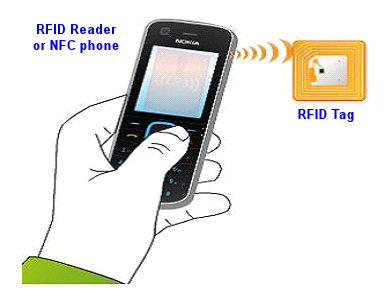
\includegraphics[width=0.4\textwidth]{readerTag.png}
      \caption{Ejemplo de interacción móvil \acs{NFC} - etiqueta.}
      \label{fig:readerTag}
    \end{center}
  \end{figure}

La interacción comienza cuando el lector se aproxima a una etiqueta
\acs{RFID}. Este emite una señal de corto alcance que es capaz de activar 
el microchip de la etiqueta y de hacer que emita los datos que contiene. En 
este caso el lector \acs{NFC} es siempre el que inicia la operación.

Pero también se permiten las comunicaciones entre dos lectores (figura
\ref{fig:mobileReader}). En este caso uno de los dos se encargará de iniciar y 
gestionar la comunicación. Existen dos modos de funcionamiento para los
dispositivos que cumplen el estándar \texttt{NFCIP-1}:

  \begin{figure}[!h]
    \begin{center}
      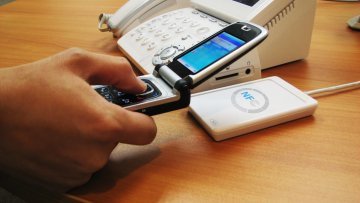
\includegraphics[width=0.5\textwidth]{mobileReader.png}
      \caption{Ejemplo de interacción móvil \acs{NFC} - lector \acs{NFC}.}
      \label{fig:mobileReader}
    \end{center}
  \end{figure}

\begin{itemize}
\item \textbf{Modo activo}:
En este modo, los dos dispositivos generan su propio campo magnético para
poder transmitir los datos. Es el modo característico de las comunicaciones
\acs{P2P} entre dispositivos (figura \ref{fig:activeMode}).

  \begin{figure}[!h]
    \begin{center}
      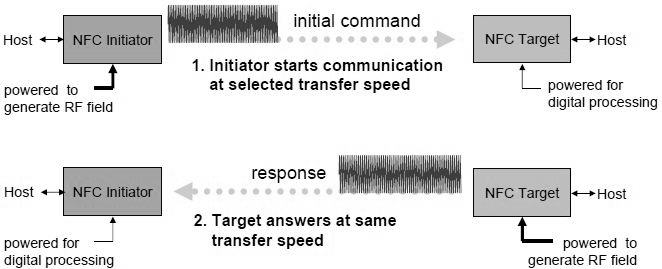
\includegraphics[width=0.8\textwidth]{activeMode.png}
      \caption{Esquema de funcionamiento del \emph{modo activo}.}
      \label{fig:activeMode}
    \end{center}
  \end{figure}

\item \textbf{Modo pasivo}:
Este modo es similar al esquema lector-etiqueta. Uno de los dispositivos
(el iniciador) genera el campo electromagnético necesario para activar al otro
y permitir la lectura de sus datos (figura \ref{fig:passiveMode}).

  \begin{figure}[!h]
    \begin{center}
      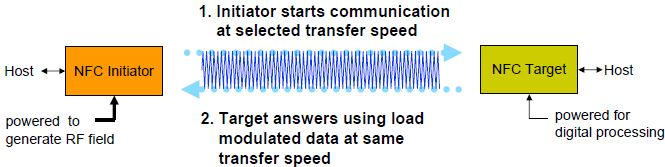
\includegraphics[width=0.8\textwidth]{passiveMode.png}
      \caption{Esquema de funcionamiento del \emph{modo pasivo}.}
      \label{fig:passiveMode}
    \end{center}
  \end{figure}
\end{itemize}

  \subsection{Características}

La tabla \ref{tab:nfcComparison} muestra una comparación entre 
las características de la tecnología \acs{NFC} y las características de 
otras tecnologías inalámbricas:

\begin{sidewaystable}[hp]
  \centering
  {\footnotesize
  \begin{tabular}{p{.12\textwidth}p{.12\textwidth}p{.12\textwidth}p{.12\textwidth}
                p{.12\textwidth}p{.12\textwidth}p{.12\textwidth}}
  \tabheadformat
  \tabhead{}   &
  \tabhead{\acs{NFC}}      &
  \tabhead{\acs{RFID}} &
  \tabhead{\acs{WiFi}} &
  \tabhead{\texttt{Bluetooth}} &
  \tabhead{\texttt{ZigBee}} &
  \tabhead{\acs{IrDA}} \\
\hline
\textit{Estándar}      & \acs{ISO}/\acs{IEC} 18092 & \acs{ISO}/\acs{IEC} 14443
                       & \acs{IEEE} 802.11         & \acs{IEEE} 802.15.1
                       & \acs{IEEE} 802.15.4       & \acs{IrDA} \\
\hline
\textit{Tasa de transferencia}
                       & 106-424 Kbps              & 106-424 Kbps
                       & 11-200 Mbps               & 1-480 Mbps
                       & 20-250 Kbps               & 1 Kbps - 100 Mbps \\
\hline
\textit{Frecuencia de utilización}
                       & 13.56 MHz                 & 13.56 MHz
                       & 2.4, 5.25, 5.6, 5.8 GHz   & 2.4 GHz
                       & 868/915 MHz, 2.4 GHz      & \\
\hline
\textit{Nº máximo de dispositivos que pueden interactuar}
                       & 2                         & 2
                       & Indefinida                & 8
                       & Indefinida                & 2 \\
\hline
\textit{Tiempo de inicialización}
                       & $<$ 0.1 ms                 & $<$ 0.1 ms
                       & $<$ 0.1 ms                 & 6 s
                       & $<$ 0.1 ms                 & 0.5 ms \\
\hline
\textit{Alcance}
                       & $<$ 20 cm                 & $<$ 3 m
                       & $<$ 100 m                 & $<$ 30 m
                       & $<$ 500 m                 & $<$ 5 m \\
\hline
\textit{Seguridad}
                       & Dada por la cercanía entre dispositivos
                       & Dada por la cercanía entre dispositivos
                       & Determinada por los mecanismos de encriptación     
                       & Determinada por los mecanismos de encriptación
                       & Determinada por los mecanismos de encriptación
                       & Dada por la cercanía entre dispositivos en línea recta \\
\hline
\textit{Consumo de energía}
                       & Mínimo o inexistente
                       & Mínimo o inexistente
                       & Alto para dispositivos alimentados por baterías
                       & Alto para dispositivos alimentados por baterías
                       & Muy bajo
                       & Bajo \\
\hline
\textit{Objetivo}
                       & Simplificar la interacción entre dispositivos
                         electrónicos          
                       & Realizar seguimiento de objetos y control de acceso
                       & Reemplazar cables en redes extensas, como las
                         \acs{LAN}
                       & Reemplazar cables para conectar dispositivos
                         electrónicos cercanos
                       & Control y monitoreo inalámbrico
                       & Reemplazar cables para conectar dispositivos
                         electrónicos cercanos \\
\hline
\textit{Ejemplo de aplicación}
                       & Intercambio de tarjetas personales electrónicas
                         acercando dos móviles
                       & Control de inventario en un supermercado
                       & Conexión entre dispositivos de una oficina (PCs,
                         impresoras, portátiles, etc.)
                       & Conexión de periféricos (teclado, ratón, etc.) a un
                         PC en la misma habitación
                       & Manejo de sistemas de riego usando sensores que
                         accionan los mecanismos correspondientes
                       & Transferencia de archivos entre un móvil y un PC \\
\hline
\end{tabular}


% Local variables:
%   coding: utf-8
%   ispell-local-dictionary: "castellano8"
%   TeX-master: "main.tex"
% End:

  }
  \caption[Comparativa entre tecnologías inalámbricas]
  {Comparativa entre tecnologías inalámbricas (~\cite{bib:nfcComparison})}
  \label{tab:nfcComparison}
\end{sidewaystable}

Como se ha comentado anteriormente, una de las principales características de 
las conexiones \acs{NFC} es que su radio de acción es muy pequeño. Esto le
permite tomar parte en operaciones que necesitan mantener seguridad en la
privacidad de los datos, como por ejemplo, para el pago de servicios. El
hecho de que el dispositivo tenga que aproximarse al terminal de pago, evita
que pueda producirse de forma accidental, que entre en conflicto con otros
terminales cercanos o que la información que se transfiere de un dispositivo
a otro pueda ser observado por un tercero.

Por otro lado, las interacciones con \acs{NFC} son rápidas e intuitivas, ya 
que estas se producen  simplemente al aproximar el dispositivo a una etiqueta 
\acs{RFID} o a otro dispositivo. Dependiendo del contenido de estos, las 
interacciones generarán acciones más complejas automáticamente en el 
dispositivo como: el inicio de una aplicación, la generación de un evento 
dentro de la aplicación, el visionado del propio contenido, el envío de un 
mensaje automático, la solicitud de un servicio a través de otro medio de 
comunicación, etc.

  \subsection{Aplicaciones}
La creciente expansión de la tecnología \acs{NFC} ha provocado el desarrollo
de múltiples aplicaciones, que buscan aprovechar las características que esta 
tecnología les ofrece para solucionar o facilitar la realización de tareas 
cotidianas.

Existe un gran número de aplicaciones, pero todas ellas pueden agruparse en
una de estas tres categorías~\cite{bib:nfcComparison}:
\begin{itemize}
\item \textbf{Inicialización de servicios}: 
En este tipo de aplicaciones, cuando un usuario toca con su dispositivo
\acs{NFC} una etiqueta \acs{RFID}, el lector extrae una serie de datos
(texto, \acs{URL}, número de teléfono, etc.) que le permiten realizar alguna
acción. Ejemplos de este tipo de aplicaciones son:
  \begin{itemize}
  \item Carteles inteligentes que promocionan un producto, servicio o evento. 
  En este caso las etiquetas proporcionan al usuario la \acs{URL} donde puede 
  obtener más información acerca de esa promoción.
  \item Etiquetas en los productos de un comercio que ofrecen más información
  acerca de dicho producto.
  \item Etiquetas ubicadas en los muebles de la casa para realizar acciones
  como controlar la iluminación o la temperatura a través del dispositivo
  móvil.
  \item Etiquetas que registran el número de visitas efectuadas por el
  personal de guardia a medida que hace el recorrido rutinario por las zonas
  del lugar.
  \item Etiquetas que facilitan operaciones simples a usuarios con alguna
  discapacidad física o mental. Por ejemplo, se puede confeccionar una agenda
  a partir de fotos de familiares a las que se adhiere una etiqueta con la
  información del número de teléfono. De esta forma cuando el usuario quiere
  llamar a alguno de sus familiares, sólo necesitará aproximar su dispositivo
  a la foto del familiar con el que quiere hablar.
  \end{itemize}
\item \textbf{Peer-to-peer}:
Este tipo de aplicaciones utilizan \acs{NFC} como mecanismo para establecer
la comunicación entre dos dispositivos que pretenden intercambiar datos. El
tráfico de dichos datos se podrá realizar mediante \acs{NFC} o mediante otra
tecnología inalámbrica (dependiendo del volumen de datos a transmitir).
Algunas de las aplicaciones que pertenecen a esta categoría son:
  \begin{itemize}
  \item Transmisión de fotos desde una cámara digital a una impresora. Cuando
  la cámara de fotos se aproxima a la impresora, se establece una comunicación
  \texttt{Bluetooth} en la que el primer dispositivo le transmite las fotos al
  segundo.
  \item Intercambio de tarjetas personales electrónicas entre dos dispositivos
  mediante la aproximación de ambos.
  \item Configuración automática de una conexión \acs{WiFi} en un lugar
  público. El usuario aproxima su dispositivo a una etiqueta que contiene la
  configuración de red y utiliza estos parámetros para iniciar automáticamente
  una conexión \acs{WiFi}.
  \end{itemize}
\item \textbf{Compras y pagos}:
Este tipo de aplicaciones dio origen a los estándares \acs{NFC}. Como ya
existían tarjetas inteligentes sin contacto para realizar pequeñas
transacciones comerciales, la tecnología \acs{NFC} tuvo que ser definida
teniendo en cuenta que fuera compatible con las aplicaciones ya existentes.
Algunos ejemplos de estas aplicaciones son:
  \begin{itemize}
  \item Pagos en parquímetros y párkings.
  \item Pago en máquinas expendedoras.
  \item Consulta de saldo en tarjetas de transporte que utilizan \acs{NFC}.
  \item \emph{Monedero electrónico}. El objetivo final es que esta tecnología
  vaya sustituyendo a las tarjetas de plástico tradicionales. De esta forma
  el usuario de un dispositivo móvil con \acs{NFC} no sólo puede utilizar su
  dispositivo para pagar en un establecimiento, sino que también puede
  mantener la información de algún sistema de fidelización o puntos de dicho
  establecimiento, los datos de la tarjeta de la seguridad social, los datos
  de los bonos del sistema de transportes de su ciudad, etc. y todo ello
  accesible a través de la tecnología \acs{NFC}.
  \end{itemize}
\end{itemize}

El número de aplicaciones sigue creciendo y cada día son más las ciudades
que disponen de servicios accesibles a través de \acs{NFC}, sobretodo en
sitios como Japón, Corea del Sur o Estados Unidos. Los fabricantes de
dispositivos móviles han observado este hecho y año tras año han ido
sacando al mercado nuevos dispositivos que incluyen esta tecnología.
Como muestra la figura \ref{fig:nfcGraph} el porcentaje de los nuevos
dispositivos que cuentan con esta tecnología se ha ido incrementando
exponencialmente.

  \begin{figure}[!h]
    \begin{center}
      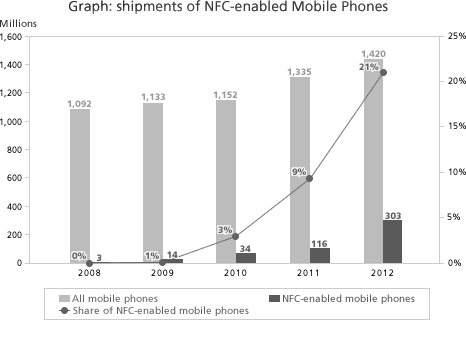
\includegraphics[width=0.8\textwidth]{nfcGraph.png}
      \caption{Evolución del número de teléfonos móviles que
      incorporan \acs{NFC}.}
      \label{fig:nfcGraph}
    \end{center}
  \end{figure}

  \subsection{El formato \acs{NDEF}}
\acs{NDEF} (\acs{NFC} Data Exchange Format) es un formato definido por el
\emph{NFC Forum} y constituye el principal estándar para el intercambio y
almacenamiento de información, pues es un formato soportado por cualquier 
dispositivo \acs{NFC}.

La estructura seguida por \acs{NDEF} posee una cabecera de datos, a partir de
la cual se encuentran los bloques de información. Cada bloque de información
se agrupa en registros que contienen a su vez los datos agrupados en mensajes
\acs{NDEF} y están caracterizados por un tipo \acs{MIME}\footnote{
\emph{Multipurpose Internet Mail Extensions} (\acs{MIME}) son una serie
de especificaciones dirigidas (en principio) al intercambio a través de
Internet de todo tipo de archivos (texto, audio, vídeo, etc.) de forma
transparente para el usuario.} definido.

Este formato tiene el inconveniente de que puede ser leido o modificado por
cualquier dispositivo \acs{NFC}, puesto que la clave empleada para el acceso
a los datos es la clave por defecto ($FF\ FF\ FF\ FF\ FF\ FF$, en hexadecimal).
Para solventar este problema, el formato \acs{NDEF} puede ser combinado con
el propuesto por \emph{MiFare}.

  \section{La tecnología \texttt{Bluetooth}}
  \label{subsec:bluetooth}
Es una especificación industrial (\acs{IEEE} 802.15.1) para redes inalámbricas
de tipo \acs{PAN} (Personal Area Network) que define un estándar global que
posibilita la transmisión de voz y datos entre diferentes dispositivos mediante
un enlace por radiofrecuencia segura.

  \subsection{Historia}
El nombre procede del rey danés y noruego del siglo X \emph{Harald Blatand},
cuya traducción al inglés sería \emph{Harold Bluetooth}, que fue conocido
por ser un buen comunicador y por unificar las tribus noruegas, suecas y
danesas.

En 1994, la empresa sueca \texttt{Ericsson} inició un estudio para investigar
la viabilidad de una nueva interfaz inalámbrica de bajo costo y consumo, para
la interconexión entre dispositivos móviles y otros objetos con el fin de
eliminar las conexiones cableadas entre ambos. A principios
de 1997, otras empresas se fijaron en los avances que \texttt{Ericsson} había
alcanzado y, un año más tarde, crearon el grupo \acs{SIG} de \texttt{Bluetooth}
(Grupo de Interés Especial en Bluetooth), formado por cinco promotores:
la propia \texttt{Ericsson}, \texttt{Nokia}, \texttt{IBM}, \texttt{Toshiba} e
\texttt{Intel}. El objetivo era definir el marco de trabajo necesario para
comenzar a comercializar dispositivos que incluyeran esta tecnología.
En la actualidad la \acs{SIG} cuenta con otros miembros como:
\texttt{Motorola}, \texttt{Lenovo} o \texttt{Microsoft}, el
respaldo de 1900 empresas de tecnología y 2000 empleados de otras tantas
empresas que investigan productos y servicios con aplicaciones
\texttt{Bluetooth}~\cite{bib:btDefinition}.

  \subsection{Características}
Al tratarse de comunicaciones por radiofrecuencia, dos o más dispositivos
pueden comunicarse vía \texttt{Bluetooth} si se encuentran dentro de un radio de
acción determinado. Este radio de acción viene determinado por la potencia de
transmisión. Según la potencia de transmisión, los dispositivos pueden
agruparse en tres clases distintas (tabla \ref{tab:btClasses}), siendo
totalmente compatibles las comunicaciones entre dispositivos
de clases distintas~\cite{bib:btDefinition}:

\begin{table}[H]
  \centering
  \caption[Clasificación de dispositivos \texttt{Bluetooth} según su potencia.]
  {Clasificación de dispositivos \texttt{Bluetooth} según su potencia.}
  \label{tab:btClasses}
  {\normalsize
  \begin{minipage}[t]{340pt}
\begin{tabular}{p{.2\textwidth}p{.24\textwidth}p{.24\textwidth}p{.24\textwidth}}
  \tabheadformat
  \tabhead{Clase} &
  \tabhead{Potencia máxima permitida (mW)} &
  \tabhead{Potencia máxima permitida (dBm\footnote{Nivel de potencia en
decibelios en relación a un nivel de referencia de 1 mW.})} &
  \tabhead{Rango\footnote{Medidas tomadas punto a punto,
tomando dos dispositivos de una misma clase instalados en campo abierto y
sin ninguna interferencia. Según condiciones ambientales usuales (como las que
se pueden dar, por ejemplo, dentro de un edificio) la distancia puede oscilar
entre 5 y 25 
metros.}} \\
\hline
\textit{Clase 1}      & 100 mW & 20 dBm & \~{}100 metros \\
\hline
\textit{Clase 2}      & 2.5 mW & 4 dBm  & \~{}25 metros \\
\hline
\textit{Clase 3}      & 1 mW   & 0 dBm  & \~{}1 metro \\
\hline
\end{tabular}
\end{minipage}

  }  
\end{table}

Cuando se deseen conectar dos dispositivos de distintos tipos, por ejemplo,
uno de clase 1 y uno de clase 2, deberán colocarse a una distancia que esté
dentro del alcance del dispositivo de clase superior, osea dentro del
rango del dispositivo de clase 2 (que tiene menor rango de actuación).

Por otro lado, la especificación \texttt{Bluetooth} ha ido evolucionando a lo
largo de los años. Desde la aparición de la versión \texttt{v1.0} en 1998,
el \acs{SIG} ha ido publicando nuevas versiones entre las que se encuentran:
la \texttt{v1.2}, que incluye compatibilidad con \acs{USB} 1.1 e 
interoperabilidad con \acs{WiFi}; la \texttt{v2.0+EDR} (2004), que mejora la 
transferencia de datos; la \texttt{v2.1}, que simplifica los pasos para crear 
conexiones entre dispositivos y permite la combinación con tecnologías como
\acs{NFC}; la \texttt{v3.0+HS} (2009), que aumenta la velocidad de
transferencia de datos; y la \texttt{v4.0} (2010), que incluye protocolos de
bajo consumo.

Cada una de las versiones ha ido mejorando aspectos clave en las comunicaciones
inalámbricas como: la posibilidad de interconectar dispositivos \emph{ad hoc},
la seguridad integrada, el bajo consumo, la facilidad de uso, el mínimo coste
y el aumento del ancho de banda (ver tabla \ref{tab:btSpeed}).

\begin{table}[H]
  \centering
  \label{tab:btSpeed}
  {\normalsize
  \begin{tabular}{p{.3\textwidth}p{.3\textwidth}}
  \tabheadformat
  \tabhead{Versión} &
  \tabhead{Ancho de banda} \\
\hline
\textit{v1.2}         & 1 Mbit/s \\
\hline
\textit{v2.0+EDR}   & 3 Mbit/s \\
\hline
\textit{v3.0+HS}    & 24 Mbit/s \\
\hline
\textit{v4.0}         & 24 Mbit/s \\
\hline
\end{tabular}

  }
  \caption[Ancho de banda soportado por las distintas versiones
  \texttt{Bluetooth}.]
  {Ancho de banda soportado por las distintas versiones \texttt{Bluetooth}.}
\end{table}

La tabla \ref{tab:nfcComparison} (página \pageref{tab:nfcComparison}) muestra
más características de la tecnología \texttt{Bluetooth} y de otras tecnologías
inalámbricas.

  \subsection{La interfaz \texttt{Bluetooth}}
Los primeros productos \texttt{Bluetooth} fueron concebidos para servir en
entornos de trabajo destinados a la gente que viaja frecuentemente. Por lo
que se empezó integrando chips de radio \texttt{Bluetooth} en portátiles,
\acs{PDA}s, móviles y auriculares. Esto originaba una serie de aspectos que
debían solucionarse~\cite{bib:btInterface}:
\begin{itemize}
\item El sistema debería poder operar en cualquier parte del mundo.
\item Puesto que está destinado a dispositivos móviles (alimentados por
baterías), el emisor de radio deberá consumir la menor energía posible.
\item La conexión deberá soportar voz y datos, y por tanto aplicaciones
multimedia.
\end{itemize}

La solución de estas premisas viene determinada por la definición de los
elementos que posibilitan las comunicaciones \texttt{Bluetooth}:

\begin{itemize}
\item \textbf{La banda de frecuencia libre} .-

Para poder operar en cualquier parte del mundo es necesario disponer de una
frecuencia de banda que esté abierta a cualquier sistema de radio,
independientemente del lugar en el que nos encontremos. Actualmente, sólo la
banda \acs{ISM} (industrial, científica y médica) de 2.45 Ghz cumple con
este requisito; y por tanto es la frecuencia elegida.

\item \textbf{Salto de frecuencia} .-

Como la banda \acs{ISM} es abierta, el sistema de radio \texttt{Bluetooth} debe
estar preparado para evitar posibles interferencias con otros sistemas de
radio. Esto lo consigue a través del método de \emph{salto de frecuencia}.
Este sistema divide la banda en varios canales de salto, donde los
transceptores\footnote{Dispositivo que realiza funciones tanto de trasmisión
como de recepción, utilizando componentes de circuitos comunes a ambas
funciones.}, durante la conexión, van cambiando de uno a otro canal de
salto de manera pseudoaleatoria. Con esto se consigue que el ancho de banda
instantáneo sea muy pequeño y tambien una propagación efectiva sobre el
total del ancho de banda. Es decir, con el sistema \texttt{FH} (salto de
frecuencia), se pueden conseguir transceptores de banda estrecha con una
gran inmunidad a las interferencias.

\item \textbf{Definición de canal} .-

El sistema \texttt{Bluetooth} utiliza un sistema \texttt{FH/TDD} (salto de
frecuencia/división de tiempo dúplex), en el que el canal queda dividido en
intervalos (llamados \emph{slots}) de 625 $\mu$s, donde cada salto de
frecuencia es ocupado por un \emph{slot} (figura \ref{fig:btChannels}). Esto
da lugar a una frecuencia de salto de 1600 veces por segundo, en el que un
paquete puede ocupar un \emph{slot} para la emisión y otro para la recepción y
que pueden ser utilizados alternativamente, dando lugar a un esquema de tipo
\texttt{TDD}.

  \begin{figure}[H]
    \begin{center}
      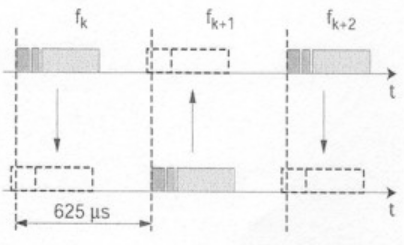
\includegraphics[width=0.6\textwidth]{btChannels.png}
      \caption{Intervalos de un canal.}
      \label{fig:btChannels}
    \end{center}
  \end{figure}

Dos o más unidades \texttt{Bluetooth} pueden compartir el mismo canal dentro
de una \emph{piconet}\footnote{Red formada por dos o más unidades
\texttt{Bluetooth} que comparten un mismo canal.}, donde una actúa como
\emph{maestra}, controlando el tráfico que se genera entre las demás unidades,
que actúan como \emph{esclavas}, enviando y recibiendo señales hacia la
unidad \emph{maestra}. El salto de frecuencia del canal está determinado por
la secuencia de la señal, es decir, por el orden en que llegan los saltos y
por la fase de esta secuencia. En \texttt{Bluetooth}, la secuencia queda fijada
por la identidad de la unidad maestra de la \emph{piconet} (un código único
para cada equipo) y por su frecuencia de reloj. Por lo que, para que una unidad
\emph{esclava} pueda sincronizarse con una unidad \emph{maestra}, debe añadir
un ajuste a su propio reloj y así poder compartir la misma portadora de salto.

  \begin{figure}[H]
    \begin{center}
      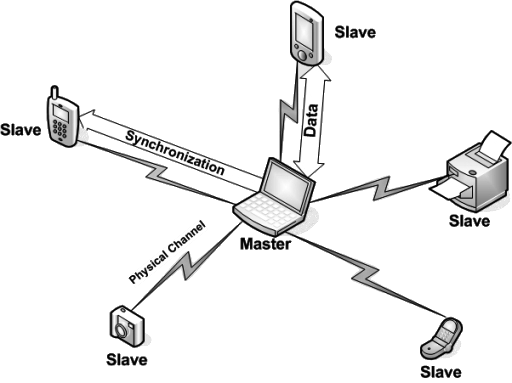
\includegraphics[width=0.7\textwidth]{btExample.png}
      \caption{Red \texttt{Bluetooth} formada por varios dispositivos. El
      portátil ejerce de \emph{maestro}.}
      \label{fig:btExample}
    \end{center}
  \end{figure}

\item \textbf{Definición de paquete} .-

La información intercambiada entre dos unidades \texttt{Bluetooth} se realiza
mediante un conjunto de \emph{slots} que forman un paquete de datos.
Cada paquete comienza con un código de acceso de 72 bits, que
determina la identidad del \emph{maestro}; seguido de la cabecera del
paquete de 54 bits, que contiene información de control como: bits de
acceso de dirección, tipo de paquete, bits de control de flujo, bits para la 
retransmisión automática de la pregunta y \emph{checksum}; y por último, el
\emph{payload} (o carga), que contiene la información y tiene una longitud de
0 a 2745 bits (ver figura \ref{fig:btPacket}).

  \begin{figure}[H]
    \begin{center}
      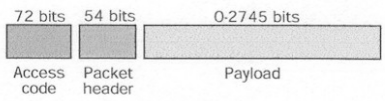
\includegraphics[width=0.5\textwidth]{btPacket.png}
      \caption{Estructura de un paquete \texttt{Bluetooth}.}
      \label{fig:btPacket}
    \end{center}
  \end{figure}

\item \textbf{Definición de enlace físico} .-

La especificación \texttt{Bluetooth} define dos tipos de enlace, que permite
soportar incluso aplicaciones multimedia:
\begin{itemize}
\item \textbf{Enlaces de sincronización de conexión orientada (SCO)}. Estos
enlaces soportan conexiones asimétricas y punto a punto y son usados
normalmente para conexiones de voz. La transmisión de voz se realiza sin
ningún mecanismo de protección.
\item \textbf{Enlaces asíncronos de baja conexión (ACL)}. Soportan
conmutaciones punto a punto simétricas o asiméticas y son usadas típicamente
para la transmisión de datos. Los datos pueden ser enviados protegidos o
sin proteger.
\end{itemize}
\end{itemize}

  \subsection{Seguridad}

Dado que los datos viajan por el medio de forma inalámbrica, es importante
asegurar la protección de esa información. Para ello se ha definido un nivel
básico de encriptación, que se ha incluido en el diseño del chip de radio
para proveer de seguridad en dispositivos que carezcan de capacidad de 
procesamiento, donde las principales medidas de seguridad son:
\begin{itemize}
\item Una rutina \emph{pregunta-respuesta}, para la autentificación.
\item Una corriente cifrada de datos, para la encriptación.
\item Y la generación de una clave de sesión (que puede ser cambiada durante
la conexión).
\end{itemize}
Los algoritmos de seguridad de \texttt{Bluetooth} trabajan con tres entidades:
la dirección de la unidad \texttt{Bluetooth}, que es una entidad pública; una
clave privada de usuario, que es una entidad secreta; y un número aleatorio,
que es diferente para cada transacción.

  \subsection{Desventajas}
  \label{subsec:disadvantages}

Aunque la \acs{SIG} sigue trabajando día a día para mejorar la tecnología
\texttt{Bluetooth}, todavía no se han terminado de solucionar algunas
limitaciones:
\begin{itemize}
\item La velocidad de transmisión es lenta para archivos pesados. Sólo a
partir de la versión (\texttt{v3.0+HS}) se han alcanzado los 24 Mbits/s.
\item El alcance es bastante limitado. Sólo los dispositivos de la
\emph{Clase 1} llega a distancias cercanas a los 100 metros.
\item Existe una limitación en cuanto a la cantidad de dispositivos que pueden
estar conectados en una misma red \texttt{Bluetooth}. El máximo es de 8
dispositivos simultáneos.
\item Si bien \texttt{Bluetooth} puede utilizarse para navegar por Internet desde
dispositivos móviles, lo cierto es que ofrece un rango de conexión muy lento,
por lo que no se recomienda ser usado para dicho fin.
\item El consumo de la batería del dispositivo aún es elevado cuando el
\texttt{Bluetooth} se encuentra activado y en \emph{modo visible}.
\item El dispositivo puede ser víctima de prácticas maliciosas como el
\emph{Bluejacking}. Esta técnica consiste en la emisión de mensajes, imágenes
u otros archivos no solicitados entre dispositivos \texttt{Bluetooth}. En
principio es una técnica inofensiva, pero provocar que el rendimiento de los
dispositivos implicados caiga.
\end{itemize}

%%%Qué es el perfil Bluetooth (donde está SPP que es lo que yo uso)?
%%%OBEX?

  \section{Los servicios web}

Un \emph{servicio web} podría definirse como un conjunto de aplicaciones o de 
tecnologías con capacidad para interoperar en la web. Estas aplicaciones o
tecnologías intercambian datos entre sí con el objetivo de ofrecer unos
servicios. Los proveedores ofrecen sus servicios como procedimientos remotos
y los usuarios solicitan un servicio llamando a estos procedimientos a través
de la web.

La interoperabilidad se consigue gracias a la adopción de estándares abiertos.
Organizaciones como \acs{OASIS}\footnote{\emph{Organization for the Advancement
of Structured Information Standards} (\acs{OASIS}) es un consorcio
internacional sin ánimo de lucro que orienta el desarrollo, la convergencia y
la adopción de estándares en el ámbito del comercio electrónico y de los
servicios web.} y \acs{W3C}\footnote{\emph{World Wide Web Consortium}
(\acs{W3C}) es un consorcio internacional que produce recomendaciones para la
\texttt{World Wide Web}.} se ocupan de definir la arquitectura y la
reglamentación de los servicios web. Además, para mejorarla, se ha creado el
organismo \texttt{WS-I}, que se encarga de desarrollar perfiles para definir
de manera más exhaustiva estos estándares.

  \subsection{Estándares empleados}
A la colección de protocolos y estándares para redes de computadores que son
utilizados para definir, localizar, implementar y hacer que un servicio web
interactúe con otro se le denomina \emph{Web Services Protocol Stack} (pila
de protocolos para servicios web). Esta colección está dividida en cuatro
áreas:
\begin{itemize}
\item \textbf{Servicio de transporte}: en este área se encuentran protocolos
como \acs{HTTP}, \acs{SMTP}, \acs{FTP} o el reciente \acs{BEEP}. Estos
protocolos son los encargados del transporte de mensajes entre aplicaciones
a través de la red.
\item \textbf{Mensajería \acs{XML}}: es el área responsable de la codificación
de mensajes en un formato común \acs{XML}, para que puedan ser entendidos
en cualquier otro extremo de una conexión de red. Algunos de los protocolos
de este área son: \texttt{XML-RPC}, \acs{SOAP} y \acs{REST}.
\item \textbf{Descripción del servicio}: está compuesta por protocolos que
describen la interfaz pública de los servicios web. El formato de interfaz
\acs{WSDL} es el más utilizado para este propósito.
\item \textbf{Descubrimiento de servicios}: se encarga de centralizar los
servicios web en un registro común en el que se publican sus localizaciones
y descripciones. Esto facilita el descubrimiento de los servicios disponibles
en la red. \acs{UDDI} es la \acs{API} más común para el descubrimiento de 
servicios.
\end{itemize}

  \subsection{Ventajas}

Una de las principales ventajas que ofrecen los servicios web es que 
proporcionan mecanismos estandarizados de comunicación entre diferentes
aplicaciones, que interactúan entre sí para presentar información dinámica al 
usuario.

Por otro lado los servicios web aportan independencia entre la 
aplicación que hace uso del servicio web y el servicio web en sí. De esta 
forma, las modificaciones realizadas en uno no deben afectar al otro.

Además, los servicios se pueden utilizar con \acs{HTTP} sobre \acs{TCP} en el 
puerto \texttt{80}. El puerto \texttt{80}, que es el utilizado por los 
navegadores, es uno de los pocos puertos que suelen estar siempre abiertos y, 
por tanto, el tráfico que discurra por ellos no va a ser bloqueado por ningún 
\emph{firewall}.

  \subsection{Funcionamiento}
La figura \ref{fig:webServices} muestra un ejemplo de funcionamiento de los
\emph{servicios web}~\cite{bib:webServices}:

  \begin{figure}[h]
    \begin{center}
      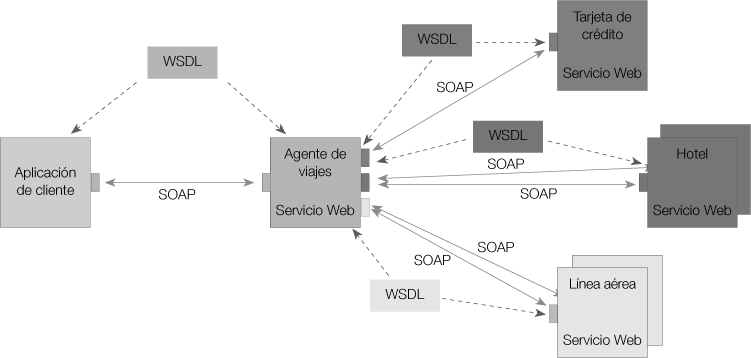
\includegraphics[width=1\textwidth]{webServices.png}
      \caption{Funcionamiento de los \emph{servicios web}.}
      \label{fig:webServices}
    \end{center}
  \end{figure}

En el ejemplo se muestra la interacción de un \emph{usuario} (que juega el
papel de cliente dentro de los servicios web) que, a través de una aplicación,
solicita información acerca de un viaje, haciendo una petición a una agencia
de viajes que ofrece sus servicios a través de Internet. Para proporcionar al
cliente la información demandada, los servicios web de la agencia solicitan a
su vez información a otros servicios web (del hotel y de la compañía aérea).
Estos devuelven la información solicitada a los servicios de la agencia para
que esta se la muestre al usuario. Por último, el usuario formaliza el pago del
viaje a través de la agencia, que servirá de intermediario entre el propio
usuario y el servicio web que gestiona el pago.

En todo el proceso intervienen varias tecnologías que hacen posible la
circulación de la información:
\begin{itemize}
\item \acs{SOAP}. Es un protocolo basado en \acs{XML}. Permite la
interacción entre los dispositivos y tiene la capacidad de transmitir
información compleja. Los datos pueden ser transmitidos a través de 
\acs{HTTP}, \acs{SMTP}, etc.

\acs{SOAP} especifica el formato de los mensajes. Un mensaje \acs{SOAP} está
compuesto por una envoltura (\emph{envolve}), cuya estructura está formada
por una cabecera (\emph{header}) y por un cuerpo (\emph{body})
(ver figura \ref{fig:soap}).

  \begin{figure}[H]
    \begin{center}
      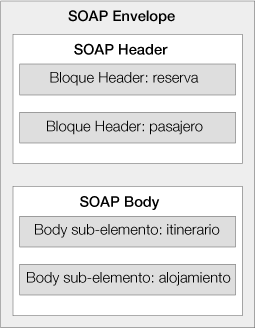
\includegraphics[width=0.4\textwidth]{soap.png}
      \caption{Estructura de los mensajes.}
      \label{fig:soap}
    \end{center}
  \end{figure}

Para optimizar el rendimiento de las aplicaciones basadas en servicios web, se 
han desarrollado tecnologías complementarias a \acs{SOAP}, que agilizan el 
envío de los mensajes (\texttt{MTOM}) y los recursos que se transmiten en estos 
(\texttt{SOAP-RRSHB}).

\item \acs{WSDL}. Es un tipo de documento que define qué hace el servicio web,
dónde se encuentra y cómo ha de ser invocado. El documento está escrito
en \acs{XML}, es procesado por el cliente y por el servicio web y, de alguna
manera, representa una especie de contrato entre el proveedor del servicio
y el que lo solicita.
\end{itemize}

Aparte de estos, se han desarrollado otros mecanismos que permiten 
enriquecer las descripciones de las operaciones que realizan los servicios 
mediante anotaciones semánticas y con directivas que definen su comportamiento.
Esto permite encontrar los servicios web que mejor se adapten a los objetivos 
deseados.

  \subsection{Arquitectura Orientada a Servicios (SOA)}
\acs{SOA} (\emph{Service-Oriented Architecture}) es un modelo de arquitectura 
que caracteriza el procedimiento para crear y usar los diversos procesos, 
reunidos en forma de servicios, que configuran un determinado \emph{proceso de 
negocio}\footnote{Conjunto estructurado de tareas, que contribuyen 
colectivamente a lograr los objetivos de una organización.}.

Esta arquitectura define y proporciona la infraestructura necesaria para que el 
intercambio de información y la participación en los procesos de negocio se 
lleven a cabo con total independencia de la plataforma sobre la que trabajan.

En la arquitectura \acs{SOA} la funcionalidad deseada se descompone en unidades
llamadas \emph{servicios}, que pueden ser distribuidos en diferentes nodos 
conectados a través de una red y que, asimismo, son combinados entre sí para 
alcanzar el resultado deseado. Estos servicios pueden proporcionar datos a 
otros o llevar a cabo actividades de coordinación entre uno o varios servicios.

La figura \ref{fig:soaElements} muestra el esquema de la arquitectura y los 
elementos que la forman~\cite{bib:soa}:

  \begin{figure}[H]
    \begin{center}
      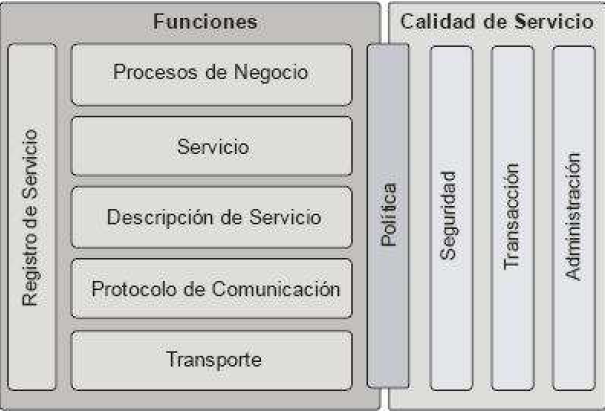
\includegraphics[width=0.8\textwidth]{soaElements.png}
      \caption{Elementos de la arquitectura \acs{SOA}.}
      \label{fig:soaElements}
    \end{center}
  \end{figure}

\begin{itemize}
\item \textbf{Funciones}:
  \begin{itemize}
  \item \textbf{Transporte}: mecanismo utilizado para llevar las peticiones
de servicio desde el consumidor hasta el proveedor de servicios y las
respuestas del proveedor hacia el consumidor.
  \item \textbf{Protocolo de comunicación}: mecanismo que pone de acuerdo
a proveedor y consumidor acerca de la naturaleza del servicio que uno solicita
y que el otro devuelve.
  \item \textbf{Descripción de servicio}: esquema que describe en qué
consiste un servicio y cómo debe invocarse.
  \item \textbf{Servicio}: describe un servicio actual que está disponible.
  \item \textbf{Procesos de negocio}: colección de servicios, invocados 
en una secuencia particular con un conjunto específico de reglas, que
satisfacen un requisito de negocio.
  \item \textbf{Registro de servicios}: repositorio de descripciones de 
servicios y datos que pueden utilizar los proveedores, para publicar sus
servicios; y los consumidores, para descubrir qué servicios están disponibles.
  \end{itemize}
\item \textbf{Calidad de Servicio}:
  \begin{itemize}
  \item \textbf{Política}: condiciones o reglas bajo las cuales un proveedor
permite el acceso a un servicio por parte de los consumidores.
  \item \textbf{Seguridad}: conjunto de reglas que pueden aplicarse para la
identificación, autorización y control de acceso a consumidores de servicios.
  \item \textbf{Transacciones}: conjunto de atributos que podrían 
aplicarse a un grupo de servicios para entregar un resultado consistente.
  \item \textbf{Administración}: conjunto de atributos que podrían 
aplicarse para manejar los servicios proporcionados o consumidos.
  \end{itemize}
\end{itemize}

Las colaboraciones en \acs{SOA} siguen el paradigma \emph{descubrir},
\emph{ligar} e \emph{invocar}, donde un consumidor realiza la localización
dinámica de un servicio consultando el \texttt{registro de servicios} para
hallar uno que cumpla con un determinado criterio. Si lo encuentra, el
registro proporciona al consumidor la interfaz de contrato y la dirección del
servicio del proveedor. La figura \ref{fig:soaRelationships} muestra las
entidades (roles, operaciones y artefactos) donde estas colaboran y sus
relaciones~\cite{bib:soa}:

  \begin{figure}[H]
    \begin{center}
      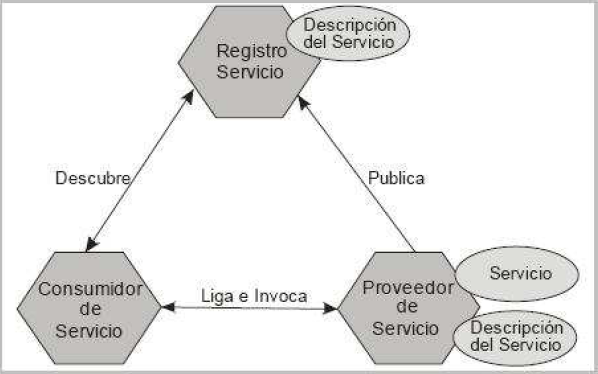
\includegraphics[width=0.8\textwidth]{soaRelationships.png}
      \caption{Relación entre las entidades en la arquitectura \acs{SOA}.}
      \label{fig:soaRelationships}
    \end{center}
  \end{figure}

Cada entidad puede desempeñar uno de estos \textbf{roles}:
\begin{itemize}
\item \textbf{Consumidor}. Es una aplicación, un módulo software u otro
servicio que demanda la funcionalidad proporcionada por un servicio y la 
ejecuta de acuerdo a un contrato de interfaz.
\item \textbf{Proveedor}. Es una entidad accesible a través de la red que 
acepta y ejecuta consultas de consumidores y publica sus servicios y su
contrato de interfaces en el \texttt{registro de servicios} para que el 
consumidor pueda descubrir y acceder a estos servicios.
\item \textbf{Registro}. Es el encargado de hacer posible el descubrimiento 
de servicios. Para ello cuenta con un repositorio de servicios disponibles que
permite visualizar las interfaces de los proveedores de servicios.
\end{itemize}

Las \textbf{operaciones} que se pueden llevar a cabo son las siguientes:
\begin{itemize}
\item \textbf{Publicar}. Antes de poder acceder a un servicio, éste ha de
publicar su descripción, para que los consumidores puedan descubrirlo e
invocarlo.
\item \textbf{Descubrir}. Un consumidor localiza un servicio que 
cumpla con un cierto criterio consultando el \texttt{registro de servicios}.
\item \textbf{Ligar e Invocar}. Una vez obtenida la descripción de un servicio 
por parte de un consumidor, éste lo invoca haciendo uso de la información 
presente en la descripción del servicio.
\end{itemize}

Y finalmente, los artefactos en \acs{SOA} son:
\begin{itemize}
\item \textbf{Servicio}. Hace referencia a cada uno de los servicios que están
disponible para el uso a través de una interfaz publicada y que permiten ser
invocados por algún consumidor.
\item \textbf{Descripción de servicio}. Se trata de la descripción de ese
servicio. La descripción especifica la forma en que el consumidor debe
interactuar con el proveedor. Normalmente especifica el formato que siguen
las consultas y las respuestas a estos, aunque también pueden especificar el
conjunto de precondiciones, postcondiciones o los niveles de calidad del
servicio (\acs{QoS}).
\end{itemize}

  \section{La tecnología \texttt{Java}}
  \label{subsec:java}
La tecnología \texttt{Java} fue diseñado por James Gosling, de \texttt{Sun 
Microsystems}, en 1990, como software para dispositivos electrónicos de
consumo, como calculadoras y microondas. Inicialmente se llamó \texttt{Oak},
aunque posteriomente tuvo que cambiar debido a que dicho nombre ya estaba
registrado por otra empresa.

La idea era crear un nuevo lenguaje lo más sencillo posible, con el objetivo
de que se pudiese adaptar con facilidad a cualquier entorno de ejecución. Por
ello, se recogieron las características esenciales que debía tener un lenguaje
de programación moderno y potente y se eliminaron todas aquellas funciones
prescindibles.

El fracaso comercial de \texttt{FirstPerson}, filial de \texttt{Sun
Microsystems} que se encargaba del desarrollo de \texttt{Oak}, llevó al
lenguaje al olvido. Tuvo que ser Bill Joy, cofundador de \texttt{Sun}, quién
le diera una segunda oportunidad al juzgar que este nuevo lenguaje podría
llegar a ser el campo de juego adecuado para disputarle a \texttt{Microsoft}
la primacía cada vez mayor en el terreno del software. Como consecuencia, se
realizaron una serie de modificaciones de diseño para adaptar al lenguaje
a su nuevo cometido y en 1995 fue presentado en sociedad como \texttt{Java}.

La tecnología \texttt{Java} está compuesta esencialmente por dos
partes~\cite{bib:java}:
\begin{itemize}
\item El lenguaje de programación \texttt{Java}.
\item La plataforma \texttt{Java}.
\end{itemize}

  \subsection{El Lenguaje de programación \texttt{Java}}
\texttt{Java} es un lenguaje de programación de alto nivel\footnote{Lenguaje
de programación que se caracteriza por expresar los algoritmos de una manera
más próxima a la capacidad cognitiva humana que a la capacidad ejecutora de
las máquinas.} y sus principales características son:
  \begin{itemize}
  \item Lenguaje orientado a objetos (\acs{OO}).
  \item Independiente de la plataforma.
  \item Capacidad multihilo.
  \item Buen rendimiento.
  \item Gran nivel de seguridad.
  \item Posee recolector de basura.
  \item Robusto e ideal para Internet.
  \item Creación de aplicaciones distribuidas.
  \item Extendido a nivel mundial e todos los ámbitos.
  \end{itemize}

Como se decía, Un programa escrito en \texttt{Java} puede ser ejecutado
independientemente de la plataforma (hardware, software o sistema operativo)
en la que se encuentre. Esto es así porque \texttt{Java} es un lenguaje en
parte \emph{interpretado}\footnote{Lenguaje de programación que está diseñado
para ser ejecutado por medio de un intérprete. Este interpreta línea
a línea cada una de las instrucciones del código fuente hasta que llega al
final o hasta que se produce un error.}, en parte \emph{compilado}
\footnote{Lenguaje de programación cuyos códigos son traducidos por medio de un 
compilador a un archivo que puede ser ejecutado en una determinada 
plataforma.}. Esto se consigue, compilando el código fuente a un lenguaje 
intermedio cercano al lenguaje máquina pero independiente al dispositivo y al 
sistema operativo en que se ejecuta. Este lenguaje resultante es el
\emph{Bytecode}(figura \ref{fig:javac}).

  \begin{figure}[H]
    \begin{center}
      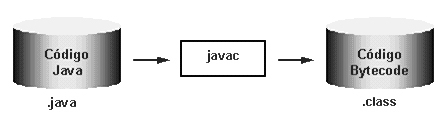
\includegraphics[width=0.8\textwidth]{javac.png}
      \caption{Compilación de código \texttt{Java} para obtener su 
      \emph{Bytecode}.}
      \label{fig:javac}
    \end{center}
  \end{figure}

Y por último, se interpreta \emph{Bytecode} por medio de un programa
denominado \emph{máquina virtual de \texttt{Java}} (\acs{JVM}) (figura
\ref{fig:jvm}), que en este caso si depende de la plataforma.

  \begin{figure}[H]
    \begin{center}
      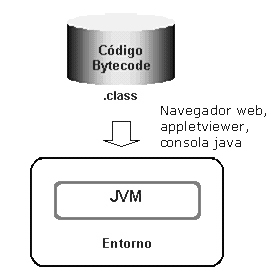
\includegraphics[width=0.4\textwidth]{jvm.png}
      \caption{Interpretación del código \emph{Bytecode}.}
      \label{fig:jvm}
    \end{center}
  \end{figure}

Esto permite que un mismo \emph{Bytecode} pueda ser ejecutado en la
\acs{JVM} de cualquier dispositivo, el ya conocido \emph{``write once, run
anywhere''}.

\subsection{La Plataforma \texttt{Java}}
La plataforma \texttt{Java} constituye el ambiente hardware y software donde
se ejecutan las aplicaciones. En la mayoría de los casos las plataformas son
descritas como la combinación de un sistema operativo y un hardware concreto.
Sin embargo, la plataforma \texttt{Java} se diferencia de estas en que es una
plataforma únicamente software y se ejecuta sobre las otras plataformas
hardware.

Así, la plataforma \texttt{Java} está compuesta por dos componentes:
\begin{itemize}
\item La máquina virtual de \texttt{Java} (\acs{JVM}). Es la base de la 
plataforma \texttt{Java} y es llevada a las diferentes plataformas hardware
para conseguir la ejecución de las aplicaciones.
\item La \acs{API} de \texttt{Java}. Es una gran colección de componentes
software y proporcionan multitud de utilidades al programador. Las \acs{API}s
están agrupadas en librerías, más conocidas como \emph{paquetes}.
\end{itemize}

Cuando una aplicación es ejecutada sobre la plataforma \texttt{Java}, tanto la
\acs{API} como la \acs{JVM} se encargan de aislar al programa de la parte
hardware.

\subsection{JavaME}
Desde su creación, la plataforma \texttt{Java} ha ido incorporando poco a poco
nuevas soluciones y servicios para atender a las necesidades que los usuarios y 
las empresas iban teniendo. Debido a la diferente naturaleza de las soluciones
propuestas, \texttt{Sun Microsystems} definió tres ediciones distintas
según el ámbito tecnológico al que estaban orientadas:

\begin{itemize}
\item \textbf{Java Standard Edition} (\acs{JavaSE}, anteriormente
\texttt{J2SE}). Edición enfocada al desarrollo de aplicaciones independientes y
\emph{applets}.
\item \textbf{Java Enterprise Edition} (\acs{JavaEE}, anteriormente
\texttt{J2EE}). Edición orientada al entorno empresarial.
\item \textbf{Java Micro Edition} (\acs{JavaME}, anteriormente \texttt{J2ME}). 
Edición adaptada al desarrollo de aplicaciones para dispositivos con recursos 
limitados.
\end{itemize}

Por lo tanto, \acs{JavaME} es una colección de tecnologías y especificaciones
que se pueden combinar para construir un completo entorno de ejecución
\texttt{Java} que se ajuste a los requisitos de un dispositivo o sector del 
mercado en particular.

La tecnología \acs{JavaME} está basada en tres elementos:
\begin{itemize}
\item La \textbf{configuración}, que proporciona el conjunto más básico de
bibliotecas y capacidades de la máquina virtual para una amplia gama de
dispositivos.
\item El \textbf{perfil}, que es un conjunto general de \acs{API}s orientadas a
las características de un tipo de dispositivo determinado.
\item Un \textbf{paquete opcional} con \acs{API}s específicas para tecnologías
específicas.
\end{itemize}

La figura \ref{fig:javaEditions} representa una visión general de los
componentes de la tecnología \acs{JavaME} y cómo se relaciona con las otras
tecnologías \texttt{Java}~\cite{bib:jmeOracle}:

  \begin{figure}[H]
    \begin{center}
      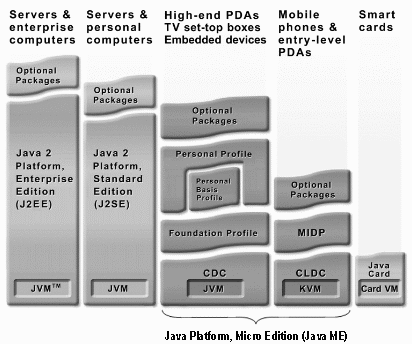
\includegraphics[width=0.7\textwidth]{javaEditions.png}
      \caption{La plataforma \acs{JavaME} dentro de la plataforma
      \texttt{Java}.}
      \label{fig:javaEditions}
    \end{center}
  \end{figure}

\subsection{Configuración}
En cuanto a la \textbf{configuración}, la plataforma \acs{JavaME} se ha
dividido en dos configuraciones básicas:
\begin{itemize}
\item La \emph{\textbf{Connected Limited Device Configuration}} (\acs{CLDC}).

Esta configuración se ha diseñado específicamente para satisfacer las
necesidades de una plataforma \texttt{Java} que funciona sobre dispositivos
con una memoria y una capacidad de procesamiento y gráfica, limitadas.
Los dispositivos que soportan \acs{CLDC} deben cumplir los siguientes
requisitos~\cite{bib:j2me}:
\begin{itemize}
  \item Disponer entre 160 KB y 512 KB de memoria total disponible. Como mínimo
se debe disponer de 128 KB de memoria \acs{ROM} para la máquina virtual
y las bibliotecas \acs{CLDC}, y 32 KB de memoria \acs{RAM} para la Máquina
Virtual en tiempo de ejecución.
  \item Procesador de 16 o 32 bits con al menos 25 MHz de velocidad.
  \item Ofrecer bajo consumo, debido a que estos dispositivos trabajan con un
suministro de energía limitado, normalmente baterías.
  \item Tener conexión a algún tipo de red, normalmente sin cable, con conexión
intermitente y ancho de banda limitado (unos 9600 bps).
\end{itemize}

Además, \acs{CLDC} aporta las siguientes funcionalidades a los dispositivos:
\begin{itemize}
  \item Un subconjunto del lenguaje \texttt{Java} y todas las restricciones
de su máquina virtual (la \acs{KVM}, de la cual se hablará en apartados
posteriores).
  \item Un subconjunto de las bibliotecas del núcleo de \texttt{Java}.
  \item Soporte para la E/S básica.
  \item Soporte para el acceso a redes.
  \item Mecanismos de seguridad.
\end{itemize}

\item La \emph{\textbf{Connected Device Configuration}} (\acs{CDC}).

Esta configuración está orientada a dispositivos con cierta capacidad
computacional y de memoria, como: decodificadores de \acs{TDT}, televisores con
Internet, algunos electrodomésticos y sistemas de navegación en automóviles.
\acs{CDC} usa una máquina virtual similar a la que posee la edición
\acs{JavaSE}, pero con limitaciones en el apartado gráfico y de memoria. Esta 
máquina virtual es la \acs{CVM} (\emph{Compact Virtual Machine}).
Los dispositivos que soportan una configuración \acs{CDC} cumplen los
siguientes requisitos~\cite{bib:j2me}:
\begin{itemize}
  \item Procesador de 32 bits.
  \item Al menos 2 MB de memoria total, incluyendo memoria \acs{ROM} y
  memoria \acs{RAM}.
  \item Poseer la funcionalidad completa de la \acs{JVM}.
  \item Conectividad con algún tipo de red.
\end{itemize}
\end{itemize}

\subsection{Perfil}
Mientras que una configuración establece las \acs{API}s que definen las 
características de una familia de dispositivos, los \textbf{perfiles} hacen
lo propio para un dispositivo concreto. Esto hace que a la hora de
desarrollar una aplicación se cuente tanto con un conjunto de \acs{API}s 
de perfil como con un conjunto de \acs{API}s de configuración.

Un perfil se construye siempre sobre una configuración determinada. Por ese
motivo, puede decirse que el perfil dota a una configuración de funcionalidad
específica.

En el apartado anterior se vio que para cada configuración se usaba una
máquina virtual específica. Esto también ocurre para los perfiles. Existen
unos perfiles que se construirán sobre la configuración \acs{CDC} y otros
que lo harán sobre \acs{CLDC}~\cite{bib:j2me}(figura \ref{fig:jmeProfiles}):

  \begin{figure}[H]
    \begin{center}
      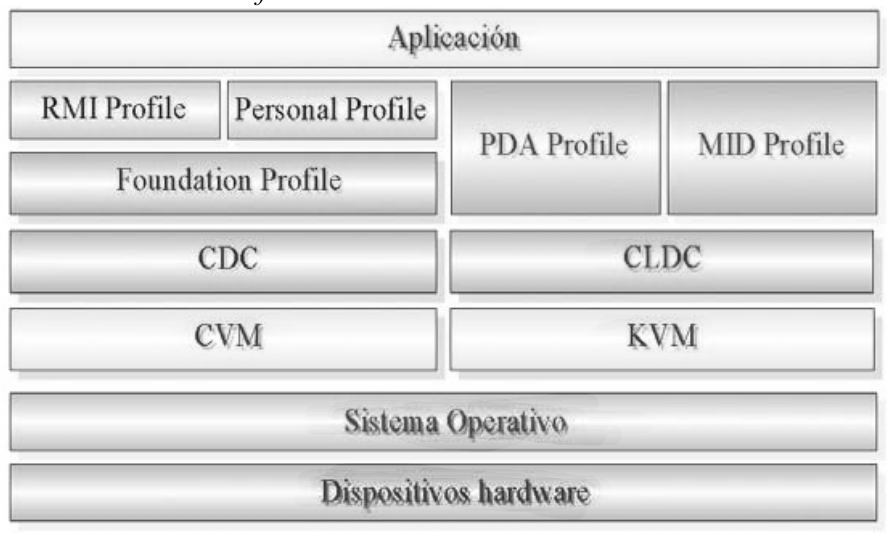
\includegraphics[width=0.8\textwidth]{jmeProfiles.png}
      \caption{Arquitectura del entorno de ejecución de \acs{JavaME}.}
      \label{fig:jmeProfiles}
    \end{center}
  \end{figure}

Para la configuración \acs{CDC} existen los siguientes perfiles:
\begin{itemize}
\item \textbf{\emph{Foundation Profile}}. 

Este perfil define una serie de \acs{API}s sobre la \acs{CDC} orientadas a
dispositivos que carecen de interfaz gráfica como, por ejemplo, decodificadores 
de \acs{TDT}.

\item \textbf{\emph{Personal Profile}}.

Es un subconjunto de la plataforma \acs{JavaSE} \texttt{v1.3}, y proporciona un 
entorno con un completo soporte gráfico \acs{AWT}. Esto permite dotar a la
configuración \acs{CDC} de una \acs{GUI} completa, con capacidades web y
soporte de \emph{applets} \texttt{Java}. Este perfil se construye sobre
la implementación del perfil \emph{Foundation Profile}.

\item \textbf{\emph{RMI Profile}}.

Soporta un subconjunto de las \acs{API}s \acs{JavaSE} \texttt{v1.3 RMI}.
Aunque algunas características de estas \acs{API}s han sido deshabilitadas
debido a las limitaciones de cómputo y memoria de los dispositivos. Este
perfil también se construye sobre la implementación del \emph{Foundation 
Profile}.

\end{itemize}

Para la configuración \acs{CLDC} por su parte, existen dos perfiles:
\begin{itemize}
\item \textbf{\emph{PDA Profile}}.

Abarca \acs{PDA}s de gama baja, con una pantalla y algún tipo de puntero
(ratón o lápiz) y una resolución de al menos 200x100 píxeles, con un factor
de 2:1.

\item \textbf{\emph{Mobile Information Device Profile} (\acs{MIDP})}.

Este es el tipo de perfil que nos interesa, pues está orientado a dispositivos 
que cuentan con las siguientes características:
\begin{itemize}
\item Reducida capacidad computacional y de memoria.
\item Conectividad limitada (en torno a 9600 bps).
\item Capacidad gráfica muy reducida (mínimo un \emph{display} de 96x54
píxeles, monocromo).
\item Entrada de datos alfanumérica reducida.
\item 128 KB de memoria \acs{ROM} para componentes \acs{MIDP}, más otros
8 KB para datos persistentes de aplicaciones.
\item 32 KB de memoria \acs{RAM} para la pila de \texttt{Java}.
\end{itemize}

El perfil \acs{MIDP} establece las capacidades del dispositivo, por lo tanto,
especifica \acs{API}s relacionadas con:
\begin{itemize}
\item Semántica y control de la aplicación \acs{MIDP}.
\item \acs{GUI}.
\item Almacenamiento persistente.
\item Trabajo en red.
\item Temporizadores.
\end{itemize}

Las aplicaciones realizadas utilizando este perfil reciben el nombre de
\emph{MIDlets} (por la adaptación libre de la palabra \emph{APPlets}). Por
lo tanto, un \emph{MIDlet} es una aplicación definida en \acs{JavaME},
construida a partir de un perfil \acs{MIDP} sobre una configuración
\acs{CLDC}.
\end{itemize}

\subsection{La máquina virtual \acs{KVM}}
Como se mencionó en apartados anteriores, cada configuración en \acs{JavaME}
disponía de su propia versión de la máquina virtual de \texttt{Java}.

En este caso, como lo que interesa es la construcción de \emph{MIDlets}, es
decir, aplicaciones con un perfil \acs{MIDP} sobre una configuración
\acs{CLDC}, va a definirse en qué consiste la máquina virtual asociada a
este tipo de aplicaciones, es decir, la máquina virtual \acs{KVM}.

\acs{KVM} es la máquina virtual más pequeña desarrollada por \texttt{Sun
MicroSystems} hasta la fecha. Su nombre proviene de \emph{Kilobyte} (por su 
escaso peso, entre 40KB y 80KB) \emph{Virtual Machine}. Originalmente, estaba 
escrita en \texttt{lenguaje C}, con aproximadamente 24000 líneas de código y 
fue diseñada para ser~\cite{bib:j2me}:
\begin{itemize}
\item Pequeña, con una carga de memoria entre los 40 y los 80 KB.
\item Altamente portable.
\item Modularizable.
\item Lo más completa y rápida posible, pero sin sacrificar las características
anteriores.
\end{itemize}

Por ello, \acs{KVM} tiene algunas limitaciones con respecto a la clásica
\acs{JVM}:
\begin{itemize}
\item No hay soporte para tipos en coma flotante.
\item No existe soporte para \acs{JNI} (\emph{Java Native Interface}).
\item No existen cargadores de clases (\emph{class loaders}) definidos por
el usuario. Sólo existen los predefinidos.
\item No se premiten los grupos de hilos. En su lugar se utilizan los
objetos \emph{Collection} para almacenar cada hilo en el ámbito de la
aplicación.
\item No existe la finalización de instancias de clases.
\item No hay referencias débiles\footnote{Un objeto que está siendo apuntado
por una referencia débil es un candidato para el recolector de basura.}.
\item Capacidad limitada en el manejo de excepciones.
\item El verificador\footnote{Es el encargado de rechazar las clases no válidas 
en tiempo de ejecución, verificando que el código no sobrepase los límites de 
la pila de la máquina virtual, comprobando que no se utilizan variables locales 
antes de ser iniciadas y comprobando que se respetan los campos, métodos y 
modificadores de control de acceso a clases.} de clases estándar de
\texttt{Java} es sustituido por un algoritmo de verificación en dos pasos 
(figura \ref{fig:preverification}) un \emph{preverificador}, durante el proceso 
de desarrollo; y un \emph{verificador} simplificado, este sí dentro de la
\acs{KVM}.

  \begin{figure}[H]
    \begin{center}
      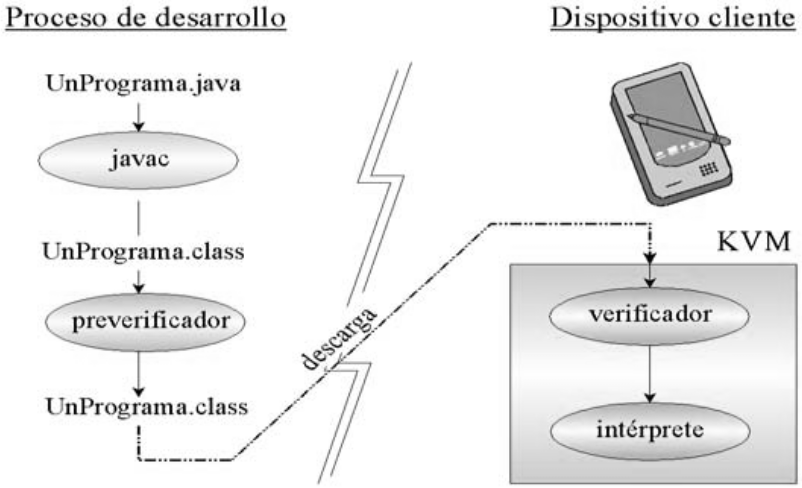
\includegraphics[width=0.8\textwidth]{preverification.png}
      \caption{Verificación de clases en \acs{CLDC}/\acs{KVM}.}
      \label{fig:preverification}
    \end{center}
  \end{figure}

\end{itemize}

\subsection{Java Specification Request}
El \emph{Java Community Process} (\acs{JCP}) es un proceso formalizado que
permite la definición, por parte de las partes involucradas, de nuevas
versiones y características de la plataforma \texttt{Java}. Este proceso
conlleva el uso de las \emph{Java Specification Request} (\acs{JSR}), es decir,
implica el uso de documentos formales que describen las especificaciones y
tecnologías propuestas para que sean añadidas a la plataforma \texttt{Java}.
Un \emph{\acs{JSR} final} (aprobado por el \emph{Comité Ejecutivo \acs{JCP}})
suministra una implementación de referencia libre de la tecnología en 
código fuente y un \emph{kit de compatibilidad tecnológica} para verificar
la especificación de la \acs{API}.

A continuación, se describen dos de las \acs{JSR}s más significativas
en el desarrollo de este \acs{PFC}:

\begin{itemize}
\item \textbf{\acs{JSR}-82} :- %(Bluetooth API)

Esta \acs{API} es conocida como \emph{Bluetooth \acs{API}} y está dividida en
dos partes totalmente independientes: el paquete
\emph{\textbf{javax.bluetooth}} y el paquete \emph{\textbf{javax.obex}}.

La primera de ellas define clases e interfaces básicas para el descubrimiento
de dispositivos y servicios, para la conexión y para las comunicaciones a bajo 
nivel, es decir, mediante flujos de datos o mediante la transimisión de cadenas
de \emph{bytes}.

El paquete \emph{javax.obex} por su parte, permite manejar el protocolo de
alto nivel \acs{OBEX} (\emph{OBject EXchange}). Este protocolo es similar
al protocolo \acs{HTTP} y permite el intercambio de archivos entre
dispositivos. En principio, \acs{OBEX} era un estándar desarrollado por
\acs{IrDA}, aunque ahora también es utilizado por otras tecnologías
inalámbricas como \texttt{Bluetooth}.

La especificación \texttt{acs{JSR}-82} está orientada principalmente al 
desarrollo de aplicaciones para la plataforma \acs{JavaME}, ya que la \acs{API} 
ha sido diseñada para depender de la configuración \acs{CLDC}. Sin embargo, 
existen también implementaciones para poder hacer uso de esta \acs{API} sobre
la plataforma \acs{JavaSE}~\cite{bib:jsr82}.

\item \textbf{\acs{JSR}-257} :- %(Contactless Communications API)

Esta \acs{API} es conocida como \emph{Contactless Communication \acs{API}} y
proporciona las librerías necesarias para implementar aplicaciones que
hacen uso de las funciones \acs{NFC} de un dispositivo móvil mediante
\acs{JavaME}.

\acs{JSR}-257 es una \acs{API} estándar de \acs{JavaME}, sin embargo, no
está incluida en el conjunto de librerías inicial del perfil \acs{MIDP}, ya
que la funcionalidad \acs{NFC} no es una característica común entre los
dispositivos móviles.

Las clases e interfaces de esta especificación se dividen en cinco
paquetes~\cite{bib:jsr257}:
\begin{itemize}
\item \emph{\textbf{javax.microedition.contactless}} :- Proporciona el 
descubrimiento de objetivos y clases comunes a todos esos objetivos.
\item \emph{\textbf{javax.microedition.contactless.ndef}} :- Contiene las 
clases e interfaces necesarias para la comunicación con etiquetas cuyo formato 
de datos es el \acs{NDEF}.
\item \emph{\textbf{javax.microedition.contactless.rf}} :- Permite las 
comunicaciones con etiquetas \acs{RFID} que no tienen un formato de datos
\acs{NDEF}.
\item \emph{\textbf{javax.microedition.contactless.sc}} :- Permite la 
comunicación con tarjetas inteligentes externas.
\item \emph{\textbf{javax.microedition.contactless.visual}} :- Permite la 
lectura y la generación de etiquetas visuales.
\end{itemize}
\end{itemize}

\section{Las pantallas táctiles}

Una pantalla táctil es una pantalla que permite la entrada de datos y órdenes 
al dispositivo mediante un toque directo sobre su superficie. Por otro lado, 
también actúa como periférico de salida, mostrándo los resultados introducidos 
previamente. El contacto puede realizarse a través del dedo (o dedos) del
usuario o con un lápiz óptico u otra herramienta similar, dependiendo de la 
tecnología empleada. Actualmente hay pantallas táctiles que pueden instalarse 
sobre una pantalla normal.

Las pantallas táctiles son populares en la industria pesada, en dispositivos
móviles y en otras situaciones donde los teclados y los ratones no permiten una 
interacción satisfactoria, intuitiva, rápida o exacta del usuario con el 
contenido.

  \subsection{Historia}
La fabricación y el uso de pantallas tactiles se ha ido extendiendo desde la 
invención de la interfaz electrónica táctil en 1971 por el Dr. Samuel C. Hurst. 
Han llegado a ser comunes en \acs{TPV}s, en cajeros automáticos y en
\acs{PDA}s, donde se suele emplear un estilete para manipular la interfaz 
gráfica de usuario y para introducir datos. La popularidad de los teléfonos 
inteligentes, las \acs{PDA}s, las \emph{tablets}, las vídeo consolas portátiles 
o de los navegadores de automóviles está generando una gran demanda y 
aceptación de las pantallas táctiles, que usan este sistema para interactuar
con el dispositivo.

En 1983, el \texttt{HP-150} fue uno de los primeros ordenadores comerciales del 
mundo que disponía de pantalla táctil. En realidad no tenía una pantalla táctil 
en el sentido propiamente dicho, sino que se trataba de una pantalla de tubo 
\texttt{Sony} de 9 pulgadas rodeada de transmisores y receptores infrarrojos 
que detectaban la posición de cualquier objeto no-transparente sobre la 
pantalla.

La mayor parte de las pantallas táctiles actuales consisten en un cristal 
transparente donde se sitúa una lámina que permite al usuario interactuar 
directamente sobre la superficie, utilizando un proyector para lanzar la 
imagen sobre la pantalla de cristal.

  \subsection{Tecnologías}

Las pantallas táctiles se implementan utilizando alguna de estas
tecnologías~\cite{bib:touchscreen}:

\begin{itemize}
\item \textbf{Resistivas}

Una pantalla táctil resistiva está formada por varias capas. Las más 
importantes son dos finas capas de material conductor entre las cuales hay una 
pequeña separación. Cuando algún objeto toca la superficie de la capa exterior, 
las dos capas conductoras entran en contacto en un punto concreto
(figura \ref{fig:resistiveTouchscreen}). De esta forma se produce un cambio en 
la corriente eléctrica que permite a un controlador calcular la posición del 
punto en el que se ha tocado la pantalla midiendo la resistencia. Algunas 
pantallas pueden medir, aparte de las coordenadas del contacto, la presión que 
se ha ejercido sobre la misma.

  \begin{figure}[h]
    \begin{center}
      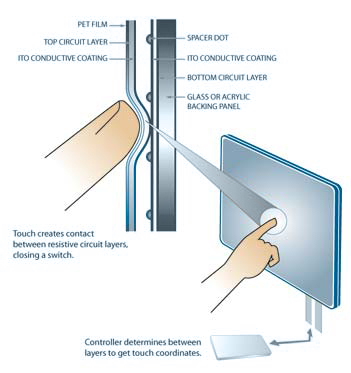
\includegraphics[width=0.6\textwidth]{resistiveTouchscreen.png}
      \caption{Pantalla táctil resistiva.}
      \label{fig:resistiveTouchscreen}
    \end{center}
  \end{figure}

Las pantallas táctiles resistivas son por norma general más accesibles pero 
tienen una pérdida de aproximadamente el 25\% del brillo debido a las múltiples 
capas necesarias. Otro inconveniente es que pueden ser dañadas por 
objetos afilados. Por el contrario, no se ven afectadas por elementos externos 
como polvo o agua, razón por la que son el tipo de pantallas táctiles más usado 
en la actualidad.

\item \textbf{Onda acústica superficial}

La tecnología de onda acústica superficial (\acs{SAW}, por sus siglas en 
inglés) utiliza ondas de ultrasonidos que se transmiten sobre la pantalla 
táctil. Cuando la pantalla es tocada, una parte de la onda es absorbida. Este 
cambio en las ondas de ultrasonidos permite registrar la posición en la que se 
ha tocado la pantalla y enviarla al controlador para que pueda procesarla
(figura \ref{fig:sawTouchscreen}).

  \begin{figure}[h]
    \begin{center}
      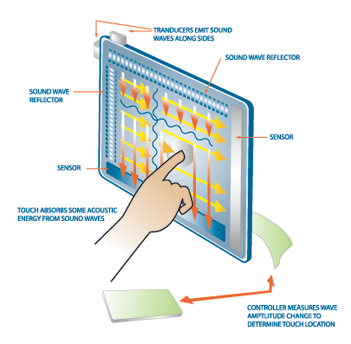
\includegraphics[width=0.8\textwidth]{sawTouchscreen.png}
      \caption{Pantalla táctil con tecnología de onda acústica
      superficial.}
      \label{fig:sawTouchscreen}
    \end{center}
  \end{figure}

\item \textbf{Capacitivas}
Una pantalla táctil capacitiva se compone de un aislante, como el vidrio, 
revestido por un conductor transparente como, óxido de indio y estaño (ITO).
Por el conductor transparente circula una corriente eléctrica continua
que es medida por un sensor. Este sensor es capaz de controlar el campo de
electrones generado tanto en el eje vertical como en el horizontal, midiendo
su capacitancia. Por otro lado, el cuerpo humano también se puede considerar un 
dispositivo eléctrico en cuyo interior hay electrones, por lo que también 
dispone de capacitancia. Cuando el campo de capacitancia normal del sensor (su 
estado de referencia) es alterado por otro campo de capacitancia, como puede 
ser el dedo de una persona, los circuitos electrónicos situados en cada esquina 
de la pantalla miden la ``distorsión'' resultante en la onda senoidal 
característica del campo de referencia y envía la información acerca de este 
evento al controlador para su procesamiento matemático (figura
\ref{fig:capacitativeTouchscreen}).

  \begin{figure}[h]
    \begin{center}
      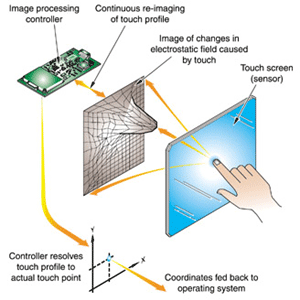
\includegraphics[width=0.6\textwidth]{capacitativeTouchscreen.png}
      \caption{Pantalla táctil capacitiva.}
      \label{fig:capacitativeTouchscreen}
    \end{center}
  \end{figure}

Por lo tanto, las pantallas táctiles capacitivas deben ser tocadas con la
mano o con los dedos, lo que evita que se vean afectadas por otros elementos
externos. Además tienen mejor claridad, sensibilidad y calidad que las
pantallas táctiles resistivas, aunque su complejo procesamiendo de la señal
hace que su coste sea más elevado.

\item \textbf{Infrarrojos}

Las pantallas táctiles por infrarrojos consisten en una matriz de sensores
(fotodetectores) y emisores infrarrojos horizontales y verticales. Los 
receptores se sitúan en los bordes de la pantalla, en ambos ejes y enfrentados
a los emisores, de tal forma que, cuando un objeto interrumpe un haz
infrarrojo vertical y otro horizontal, quedan registradas las coordenadas
donde el objeto ha hecho contacto (figura \ref{fig:irTouchscreen}).

  \begin{figure}[h]
    \begin{center}
      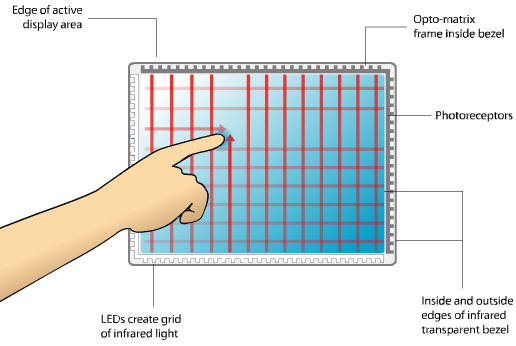
\includegraphics[width=0.8\textwidth]{irTouchscreen.png}
      \caption{Pantalla táctil por infrarrojos.}
      \label{fig:irTouchscreen}
    \end{center}
  \end{figure}

Este tipo de pantallas son muy resistentes por lo que son utilizadas 
en muchas de las aplicaciones militares que exigen una pantalla táctil.
Por otro lado, tienen el inconveniente de que son sensibles a la 
suciedad y el polvo; y pueden sufrir paralelaje\footnote{Cuando el marco
(donde se sitúan los emisores y receptores) o la pantalla se desvían de su 
posición original, por un golpe por ejemplo, el usuario notará que las 
coordenadas que selecciona no corresponden con las coordenadas que quedan
marcadas en la pantalla.}.

\item \textbf{Imagen óptica}

Es un desarrollo relativamente moderno, en el que dos o más cámaras son 
situadas alrededor de la pantalla, habitualmente en las esquinas. Por otro 
lado, varios emisores de infrarrojos son situados en el campo de visión de las
cámaras, a lo largo de los lados no ocupados por las cámaras. Un toque en la 
pantalla muestra una sombra de forma que cada par de cámaras puede 
triangularizarla para localizar el punto exacto de contacto. Esta tecnología 
está ganando popularidad debido a su escalabilidad, versatilidad y su precio, 
especialmente para pantallas de gran tamaño (figura \ref{fig:oiTouchscreen}).

  \begin{figure}[h]
    \begin{center}
      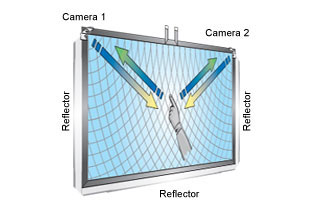
\includegraphics[width=0.6\textwidth]{oiTouchscreen.png}
      \caption{Pantalla táctil a través de imagen óptica.}
      \label{fig:oiTouchscreen}
    \end{center}
  \end{figure}

\item \textbf{Tecnología de señal dispersa}

Este sistema utiliza sensores que detectan la energía mecánica que se produce
en el cristal de la pantalla tras el contacto con algún objeto (figura
\ref{fig:dispersiveTouchscreen}). Unos algoritmos complejos se encargan de 
interpretar esta información para obtener el punto exacto del contacto.

  \begin{figure}[h]
    \begin{center}
      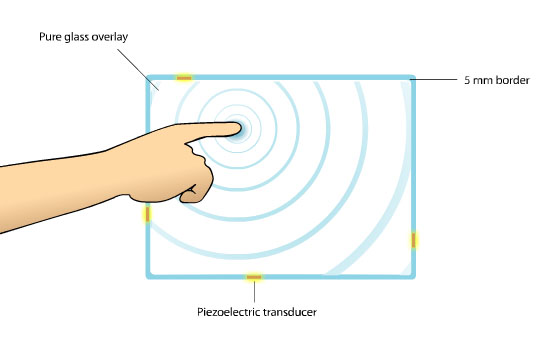
\includegraphics[width=0.8\textwidth]{dispersiveTouchscreen.png}
      \caption{Pantalla táctil con tecnología de señal dispersa.}
      \label{fig:dispersiveTouchscreen}
    \end{center}
  \end{figure}

Esta tecnología es resistente al polvo y otros elementos externos, incluidos 
arañazos y proporciona unos excelentes niveles de claridad. Además, como 
el contacto es detectado a través de vibraciones mecánicas, cualquier objeto 
puede ser utilizado para producir estos eventos, incluyendo el dedo o la uña. 
Un efecto lateral negativo de esta tecnología es que tras el contacto inicial 
el sistema no es capaz de detectar un dedo u objeto que se encuentre parado 
tocando la pantalla.

\item \textbf{Reconocimiento de pulso acústico}

Estos sistemas utilizan cuatro transductores piezoeléctricos, situados cada uno 
en uno de los lados de la pantalla, para convertir la energía mecánica del 
contacto en una señal electrónica (figura \ref{fig:acousticTouchscreen}). 
Después, esta señal es convertida en una onda de sonido y es comparada con
una lista de sonidos pregrabados con todas las posiciones del cristal.

  \begin{figure}[h]
    \begin{center}
      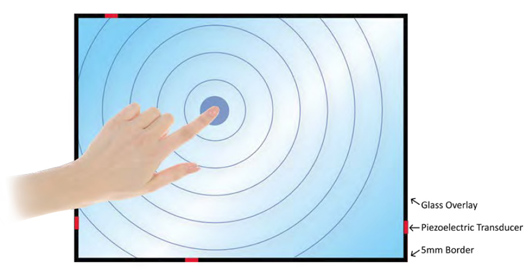
\includegraphics[width=0.8\textwidth]{acousticTouchscreen.png}
      \caption{Pantalla táctil por reconocimiento de pulso acústico.}
      \label{fig:acousticTouchscreen}
    \end{center}
  \end{figure}

En este sistema la pantalla táctil es completamente de cristal y no necesita 
ningún otro objeto especial para su utilizacion, por lo que la buena óptica y 
la durabilidad están garantizadas. Además, también tiene la ventaja de que
puede funcionar con arañazos o polvo sobre la pantalla y tiene unos altos
niveles de precisión.
\end{itemize}

  \subsection{Especificaciones \acs{HID}}

Las pantallas táctiles se encuentran definidas dentro de la especificación de 
dispositivos \acs{HID} (dispositivos de interfaz humana) como digitalizadores, 
junto con dispositivos como los \emph{touchpads} y las tabletas digitalizadoras 
entre otros.
 
Esta especificación incluye los campos utilizados para el manejo de este tipo 
de dispositivos. Algunos de los más interesantes son:
\begin{itemize}
\item \textbf{\emph{Tip Pressure}}: que representa la fuerza por un 
transductor, habitualmente un estilete o también un dedo.
\item \textbf{\emph{Barrel Pressure}}: fuerza que ejerce el usuario en el 
sensor del transductor, como por ejemplo un botón sensible a la presión en el 
puntero de manejo.
\item \textbf{\emph{In Range}}: que indica que el transductor se encuentra en 
el área donde la digitalización es posible.
\item \textbf{\emph{Touch}}: indica si un dedo está tocando la pantalla. El 
sistema suele interpretarlo como un \emph{clic} de botón primario.
\item \textbf{\emph{Untouch}}: indica que el dedo ha perdido contacto con la 
superficie de la pantalla. Se interpreta como la acción de soltar el botón 
primario.
\item \textbf{\emph{Tap}}: indica que se ha realizado un toque con el dedo en 
la pantalla, levantándolo rápidamente sin prolongar el contacto. Se interpreta 
como un evento provocado por un botón.
\end{itemize}

\section{La computación móvil}
\emph{Computación móvil} es un término utilizado para designar a la interacción
hombre-máquina a través de un dispositivo que debe ser transportado por el
usuario durante su uso, normalmente por la naturaleza del trabajo que el hombre
y la máquina desempeñan. La computación móvil trata de responder a los 
problemas asociados con las comunicaciones, el hardware y el software que
los dispositivos necesitan para llevar a cabo este tipo de computación.
Uno de los aspectos más importantes es que los dispositivos deben facilitar el
acceso a la información que el usuario pueda demandar, por lo que, el
dispositivo debe estar dotado de alguna tecnología que lo conecte con el
exterior.

  \subsection{Evolución}
En los años 60 y 70, no existía la computación personal y los grandes centros
de cómputo eran los responsables del manejo de toda la información, desde
el proceso de entrada de datos, hasta el procesado, la validación y la
impresión de la información. Los usuarios directos de dicha información no
tomaban parte en el proceso de captura ni en el de procesado, sólo tomaban
parte de su utilización.

En los 80 y 90, empezó a hacerse común la utilización de los ordenadores
personales, los cuales facilitaban que el propio usuario fuera el responsable
de la introducción de los datos de entrada, del procesado y de la utilización
de la información generada. Pero había un problema, cuando la información no
se generaba cerca del terminal que iba a procesar los datos se hacía necesaria
una toma de datos ``manual'' y una posterior digitalización de dichos datos.
Esto ralentizaba el proceso y aumentaba la probabilidad de errores en la
transcripción~\cite{bib:micMobileComputing}.

La computación móvil, nació con la vocación de acabar con este tipo de 
problemas. Para ello, se establecieron los siguientes
objetivos~\cite{bib:ticUTP}:
\begin{enumerate}
\item La primera fase consistía en hacer dispositivos lo suficientemente
pequeños como para poder ser transportados fácilmente. Es decir, dispositivos
móviles.
\item La segunda fase trataba de reemplazar los cables de comunicación por
medios inalámbricos.
\item Y la tercera fase era una combinación de las dos primeras, es decir,
consistía en potenciar la utilización de dispositivos móviles en un entorno
inalámbrico. Esta combinación permite las conexiones en tiempo real entre
dispositivos móviles y otros dispositivos de computación.
\end{enumerate}

  \subsection{Características}
La computación móvil posee dos características principales~\cite{bib:ticUTP}:
\begin{itemize}
\item \textbf{Movilidad}. Implica la portabilidad basada en el hecho de que
los usuarios llevan un dispositivo móvil a todas partes. Estos dispositivos
deben permitir una comunicación en tiempo real con otros sistemas,
independientemente del lugar en el que se encuentren.
\item \textbf{Amplio alcance}. La computación móvil debe ser accesible a todas
las personas, de tal forma que todos puedan beneficiarse de su uso.
\end{itemize}

Además, la computación móvil puede enriquecerse incorporando los siguientes
atributos:
\begin{itemize}
\item \textbf{Ubicuidad}. Se refiere a la cualidad de estar disponible en
cualquier momento y en cualquier lugar.
\item \textbf{Comodidad}. Si los clientes son capaces de realizar una gran
parte de sus gestiones a través de su dispositivo móvil y de una forma cómoda,
repetirán este proceso de forma habitual.
\item \textbf{Conectividad instantánea}. La conectividad instantánea a redes
como Internet proporciona a los usuarios el acceso a la información que les
interesa independientemente de dónde se encuentren.
\item \textbf{Personalización}. Se refiere a la cualidad de poder elegir
la forma en la que los dispositivos presentan la información a los consumidores
individuales.
\item \textbf{Localización}. Conocer la ubicación física de los usuarios en
cualquier momento es clave a la hora de ofrecerles productos y servicios.
\end{itemize}

  \subsection{Limitaciones}
La naturaleza intrínseca de los dispositivos que posibilitan la computación 
móvil está acompañada de una serie de limitaciones que, por fortuna, van
atenuándose con el desarrollo de nuevas tecnologías y materiales. Estas
limitaciones son~\cite{bib:wikiMobileComputing}:
\begin{itemize}
\item \textbf{Ancho de banda}: el acceso a Internet a través de tecnologías
inalámbricas como \acs{GPRS} o \acs{EDGE}, o más recientemente con redes
\texttt{3G}\footnote{Es la abreviación de tercera generación de transmisión de 
voz y datos a través de telefonía móvil mediante \texttt{UMTS} (\emph{Universal 
Mobile Telecommunications System}). Proporcionan la posibilidad de transferir 
tanto voz y datos (una llamada telefónica o una videollamada) como datos no-voz 
(como la descarga de programas, intercambio de correos electrónicos, y 
mensajería instantánea).}. Estas redes están disponibles generalmente dentro
del alcance de las antenas comerciales de telefonía móvil.
\item \textbf{Seguridad}: la conectividad de los dispositivos móviles está
en ocasiones condicionada al uso de las redes públicas, por lo que se
recomienda un uso cuidadoso de las redes \acs{VPN}\footnote{Tecnología de red
que permite una extensión de la red local sobre una red pública o no
controlada.}, ya que es fácil atacar redes \acs{VPN} a través del gran número
de redes interconectadas que comparten un mismo medio.
\item \textbf{Consumo de energía}: cuando no es posible conectar el dispositivo
a una fuente de alimentación o a un generador portátil, la autonomía de dicho
dispositivo depende exclusivamente de la duración de su batería. Por otro lado,
la batería debe ser lo suficientemente pequeña como para que pueda ser
compactada dentro del dispositivo y a la vez, lo suficientemente grande o
eficiente como para que pueda satisfacer las necesidades del dispositivo
durante un tiempo razonable, según el cometido de dicho dispositivo.
\item \textbf{Interferencias}: el clima, el terreno o la lejanía del punto de
emisión más cercano pueden afectar a la recepción de la señal del dispositivo.
La recepción en túneles, algunos edificios y zonas rurales suele ser pobre.
\item \textbf{Riesgos potenciales de salud}: en algunos países el uso de
dispositivos móviles miestras se conduce un vehículo todavía no está
penalizado. Este hecho aumenta la probabilidades de que el usuario se vea
involucrado en un accidente de tráfico. Por otro lado, existen estudios que
pretenden demostrar que las radiaciones que emiten los teléfonos móviles 
pueden afectar a la salud de sus usuarios.
\item \textbf{Interfaz del dispositivo}: las pantallas y teclados de los
dispositivos suelen ser pequeños y esto puede desembocar en un problema de
usabilidad, sobretodo para ciertos usuarios (como personas mayores).
Para solucionar esto, se proponen métodos alternativos para la entrada de
datos, como el reconocimiento de voz o el reconocimiento de escritura.
\end{itemize}

  \subsection{Dispositivos}
Las principales categorías de dispositivos que pertenecen al mundo de la
computación móvil son las siguientes~\cite{bib:wikiMobileComputing}:
\begin{itemize}
\item \textbf{Ordenador portátil}. Es un ordenador de propósito general
que puede transportarse fácilmente de un lugar a otro, pero no puede utilizarse 
mientras tanto pues, por su tamaño, necesita ser apoyado en alguna superficie 
estable. Además, su batería no proporciona una autonomía de más de unas pocas
horas.
\item \textbf{\emph{Tablet PC} (tableta digital)}. Es un ordenador que carece 
de teclado. En su lugar tiene una pantalla táctil con la que el usuario 
interactúa. Puede realizar la mayor parte de las taréas de un ordenador 
portátil común, pero no es muy adecuado para tareas que requieran un uso 
intensivo del teclado, puesto que el teclado táctil disminuye notablemente el 
espacio en pantalla de la aplicación activa.
\item \textbf{\acs{PDA} (\emph{Personal Digital Assistant})}. Es un
ordenador de tamaño de bolsillo, que tiene funcionalidades limitadas. Su
objetivo es sincronizar su información con la de un ordenador de escritorio
en tareas como: la administración de la agenda de contactos, la revisión de
notas o la gestión del correo electrónico, entre otras.
\item \textbf{\emph{Internet appliance} (Dispositivo para Internet)}. Es un 
dispositivo similar a una \acs{PDA}, pero con funcionalidad multimedia. No 
tiene el poder de computación de un \emph{tablet PC} pero cuenta con 
aplicaciones como: un reproductor de \texttt{MP3} y vídeo, un navegador web, 
una aplicación de \emph{chat} o un visor de imágenes (figura
\ref{fig:internetApp}).

  \begin{figure}[h]
    \begin{center}
      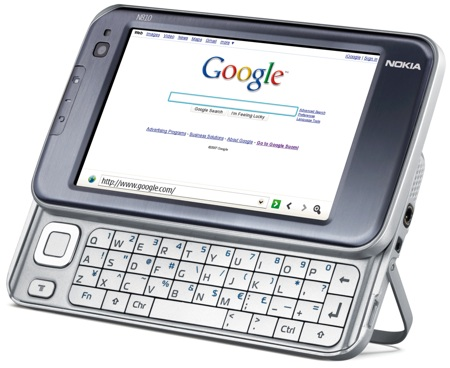
\includegraphics[width=0.4\textwidth]{internetApp.png}
      \caption{El \texttt{Nokia 810} es un dispositivo de la clase
      \emph{Internet appliance}.}
      \label{fig:internetApp}
    \end{center}
  \end{figure}

\item \textbf{\acs{UMPC} (\emph{Ultra Mobile Personal Computer})}. Es una
dispositivo del tamaño de una \acs{PDA}, que cuenta con una completa 
\emph{suite} de aplicaciones que se ejecutan sobre un sistema operativo de 
propósito general (figura \ref{fig:umpc}).

  \begin{figure}[h]
    \begin{center}
      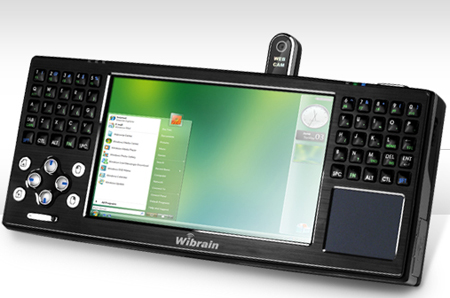
\includegraphics[width=0.5\textwidth]{umpc.png}
      \caption{El \texttt{Wibrain B1} es un dispositivo del tipo \acs{UMPC}.}
      \label{fig:umpc}
    \end{center}
  \end{figure}

\item \textbf{\emph{Smartphone} (teléfono inteligente)}. Es un teléfono móvil 
construido sobre una plataforma informática móvil, con una mayor capacidad de 
computación y conectividad que un teléfono móvil convencional.
\item \textbf{\emph{Carputer}}. Es el término utilizado para describir una 
categoría de computadora portátil utilizada o modificada específicamente para 
ser instalada en automóviles. Controla funcionalidades como: el reproductor
de música, el reproductor de DVDs, la conectividad \texttt{Bluetooth} o
el \acs{GPS} (figura \ref{fig:carputer}).

  \begin{figure}[h]
    \begin{center}
      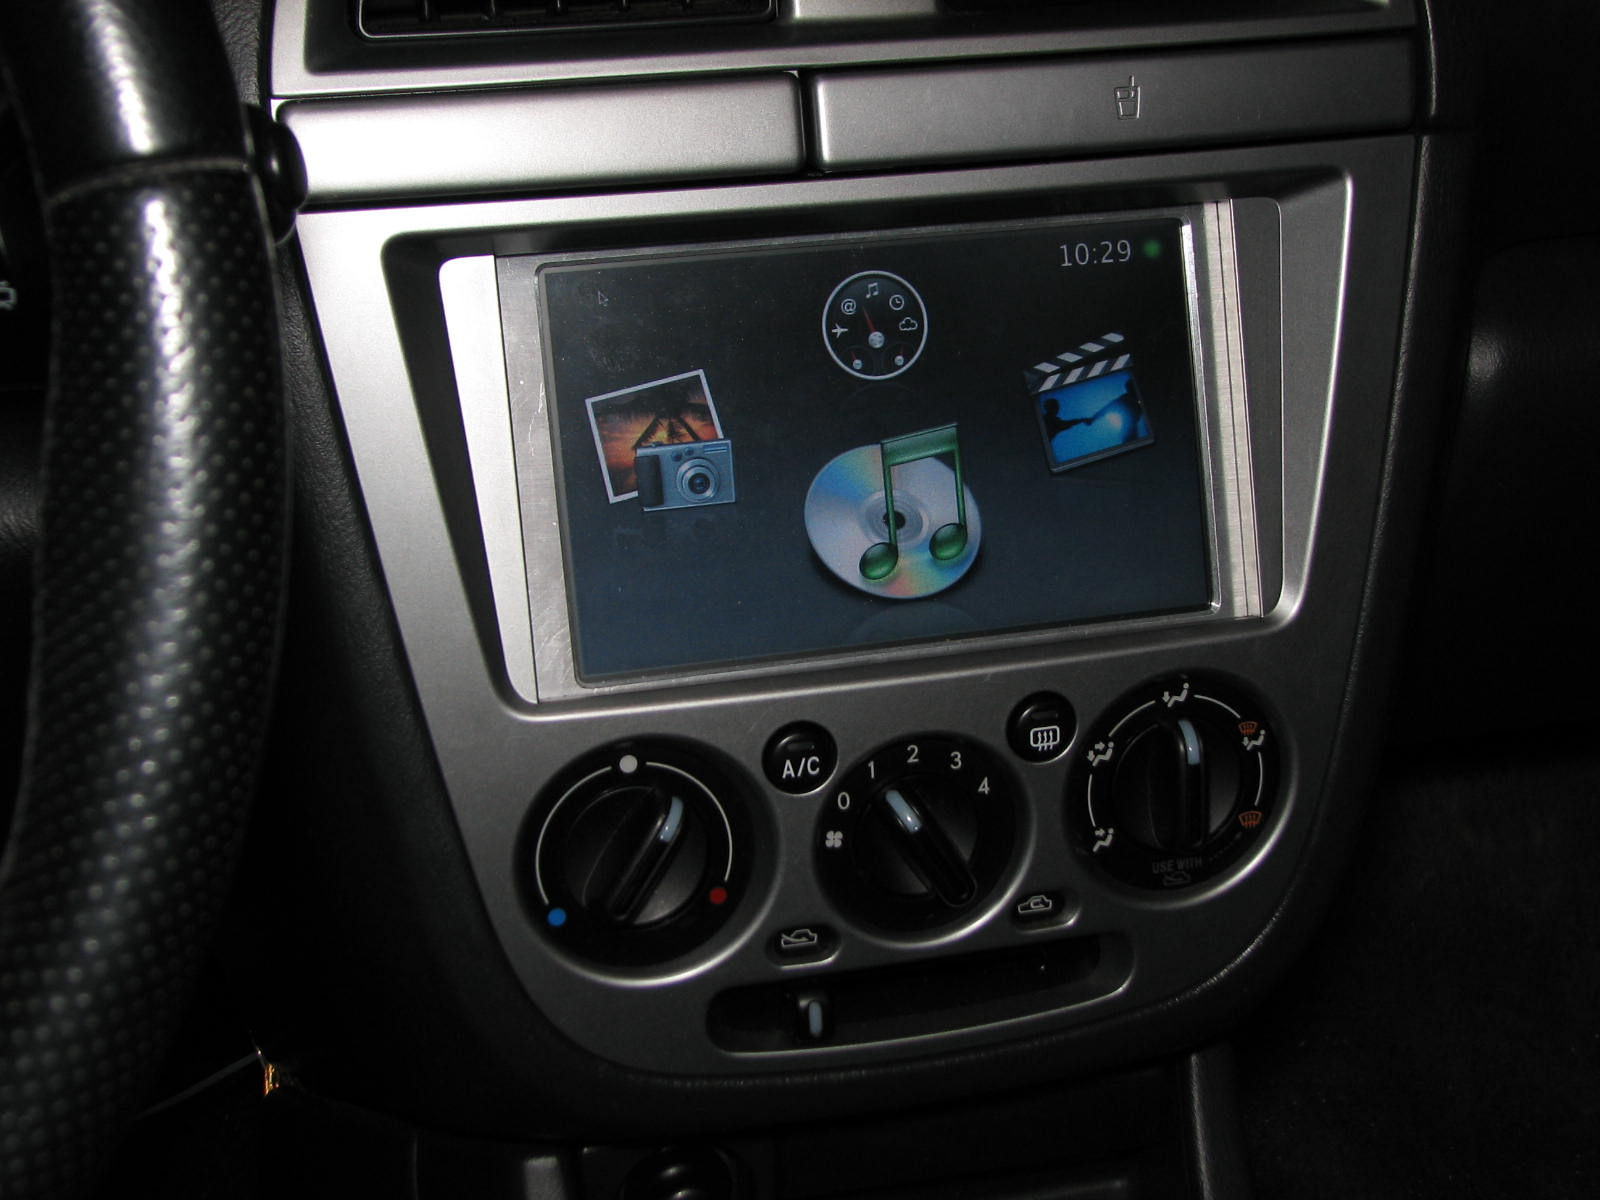
\includegraphics[width=0.5\textwidth]{carputer.png}
      \caption{\emph{Carputer} que permite varias funcionalidades multimedia.}
      \label{fig:carputer}
    \end{center}
  \end{figure}

\item \textbf{\emph{Pentop computer}}. Es un dispositivo de computación del
tamaño y la forma de un bolígrafo, que funciona como un bolígrafo y además,
como un reproductor de \texttt{MP3}, un dispositivo de almacenamiento digital,
un traductor de idiomas o una calculadora (figura \ref{fig:pentop}).

  \begin{figure}[h]
    \begin{center}
      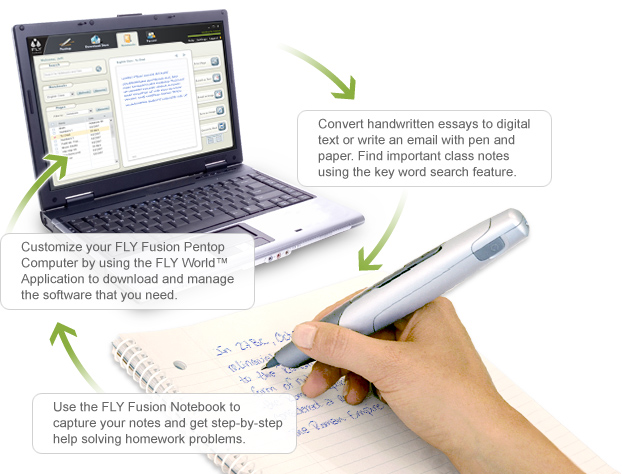
\includegraphics[width=0.8\textwidth]{pentop.png}
      \caption{\texttt{Pentop FLY Fusion}. Permite, entre otras cosas, 
      capturar y digitalizar lo que se está escribiendo para posteriormente
      convertirlo en texto en el PC.}
      \label{fig:pentop}
    \end{center}
  \end{figure}

\end{itemize}
Los límites que separan unas categorías de otras son borrosos y, a veces, un
dispositivo puede pertenecer, por ejemplo, a una categoría según su tamaño o
su hardware y a otra según su funcionalidad.

  \subsection{Aplicaciones}
Los dispositivos anteriormente mencionados dan soporte a una serie de
aplicaciones que han aparecido gracias a evolución de estos.
Algunas de las aplicaciones más importantes son~\cite{bib:micMobileComputing}:
\begin{itemize}
\item \textbf{Seguimiento de pacientes}: la computación móvil permite al
médico mantener un contacto directo con su paciente. Y esto no se limita
al envío o recepción de mensajes (hablados o escritos), sino que incluye
también el monitoreo constante de los signos vitales que son objeto de dicho
seguimiento.
\item \textbf{Ventas directas}: gracias a la computación móvil es posible
consultar inventarios y realizar pedidos de forma inmediata. Esto ha favorecido
que muchas empresas hayan apostado por un modelo de negocio basado en la
venta a través de Internet.
\item \textbf{Servio a clientes}: la asesoría de un servicio técnico es un
área en donde la computación móvil es vital. La consulta a bases de datos
inteligentes, el acopio de información actualizada y la consulta a
especialistas, es sólo una pequeña muestra de todo lo que puede impactar
esta tecnología.
\item \textbf{Profesionales viajeros}: la computación móvil permite:
tener localizados a los miembros de una plantilla, asignarles nuevas tareas,
actualizar las tareas activas con sus aportaciones, etc. independientemente
de que el/los miembro/s estén en su puesto de trabajo habitual o no.
\item \textbf{Manejo de sucursales}: en un mundo en el que las empresas han
dejado de tener una sola oficina para expandirse, las sucursales aparecen casi
sin desearlo, con una gran cantidad de datos que deben cruzarse de forma rápida 
y segura.
\item \textbf{Grupos de trabajo}: cada vez es más común afrontar proyectos
con un personal muy especializado, el cual no siempre trabaja bajo un mismo
techo y, en ocasiones, ni siquiera en la misma ciudad o país.
\end{itemize}

Algunas de estas categorías han evolucionado muy rápidamente, gracias a la
competitividad existente entre las compañías que han apostado fuerte por el
desarrollo de ese tipo servicios.

  \section{Estudios relacionados}
  \label{subsec:related}
En la siguiente sección se hará un repaso de algunos de los trabajos de
investigación más relevantes en el campo de los modelos de negocio orientados
al uso de la tecnología \acs{RFID} y \acs{NFC}.

    \subsection{Modelos de comercio utilizando NFC}
  Los servicios que ofrece \acs{NFC} están muy diversificados y extendidos
  por todo el mundo. Algunos de los servicios están orientados a utilizar
  las tarjetas inteligentes como un monedero electrónico sustitutivo del
  pago en efectivo en los medios de transporte público, otros sustituyen
  a los clásicos cupones para premiar la fidelidad de los clientes de un
  establecimiento, otros sirven para solicitar un servicio de entre una
  lista de servicios disponibles (como elegir un producto dentro de una
  lista de productos), etc.

  Con el fin de integrar todos estos servicios como un proceso común de
  comercio electrónico basado en NFC, se ha propuesto un modelo genérico
  para el comercio móvil basado en \acs{NFC} (o \acs{NMC}, por sus siglas
  en inglés)~\cite{bib:nfcCommerce}. Este modelo caracteriza los problemas y
  las tecnologías que intervienen en cada una de las siguientes fases
  (figura \ref{fig:nmcModel}):

  \begin{figure}[!h]
    \begin{center}
      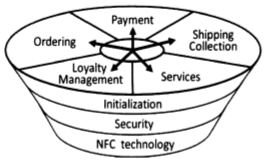
\includegraphics[width=0.5\textwidth]{nmcModel.png}
      \caption{El modelo \acs{NMC}.}
      \label{fig:nmcModel}
    \end{center}
  \end{figure}

  \begin{itemize}
  \item \textbf{Fase de inicialización}. Para la construcción de un servicio
  de comercio basado en \acs{NFC} se necesitan definir cuatro componentes
  fundamentales:
    \begin{itemize}
    \item \textbf{Servicio de \emph{back-end}}\footnote{En diseño de software
    el \emph{front-end} es la parte del software que interactúa con el o los
    usuarios y el \emph{back-end} es la parte que procesa la entrada desde el
    \emph{front-end}} \textbf{basado en \acs{NFC}}. Este
    servicio es el responsable de todo el intercambio de información durante
    el proceso de comercio. Está gestionado por el proveedor de servicios
    basados en \acs{NFC}.
    \item \textbf{Aplicación de terminal genérico (\acs{GTA})}. Como el tamaño
    de la memoria del dispositivo móvil es limitada, combiene definir una
    aplicación genérica que permita realizar todas las gestiones comerciales.
    \item \textbf{Funcionalidad de las etiquetas}. Definir los tipos de
    etiquetas que se utilizarán para construir un entorno de servicios con
    \acs{NFC} que siga el estándar \acs{NDEF}. Por ejemplo, un tipo de etiqueta
    para iniciar la aplicación, otro para cada uno de los productos, otro
    para seleccionar descuentos y otro para seleccionar el servicio.
    \item \textbf{Habilitar el servicio \acs{NFC}}. La etiqueta de inicio de
    aplicación se encargará de cargar el \acs{GTA} y de arrancar el servicio de
    \emph{back-end}, para que el usuario pueda usarlos nada más iniciar la
    aplicación.
    \end{itemize}
  \item \textbf{Fase de pedido}. Después de la inicialización el cliente ya
  está preparado para realizar un pedido a través de un catálogo de productos:
    \begin{itemize}
    \item Cada \textbf{catálogo} tiene una o varias etiquetas que representan
    los productos ofrecidos por el servicio. Cuando el dispositivo toca una
    de estas etiquetas, la aplicación puede llamar al servicio \emph{back-end}
    para descargar el contenido (imágenes, videos, etc.) relacionado con el
    contenido del producto al que representa la etiqueta.
    \item Además, cada producto puede tener opciones del tipo \emph{sabor},
    \emph{volumen}, \emph{tamaño}; que pueden ser seleccionables a través
    de otras etiquetas o a través de la pantalla del dispositivo.
    \end{itemize}
  \item \textbf{Fase de pago}. Hay dos métodos de pago disponibles en el
  modelo \acs{NMC}:
    \begin{itemize}
    \item \textbf{Modo monedero electrónico} (figura \ref{fig:e-wallet}). 
    Después de que el cliente haya realizado un pedido, el \acs{GTA} 
    solicitará la información del producto al servicio \emph{back-end}. Si el 
    servicio \emph{back-end} confirma la autenticidad del usuario y de la 
    operación, le devolverá al \acs{GTA} el importe del producto. Esta 
    cantidad será decrementada del monedero electrónico. El monedero 
    electrónico es un elemento seguro al que sólo se puede acceder con el 
    permiso del servicio \emph{back-end}. Los clientes deben disponer de saldo 
    para poder realizar un pedido (método prepago).

    \begin{figure}[!h]
      \begin{center}
        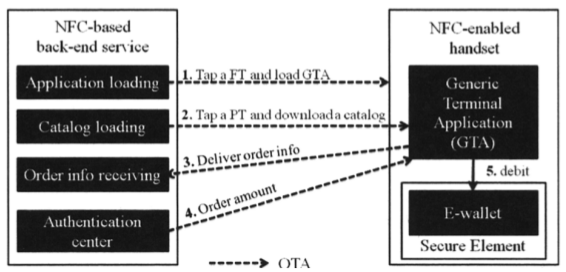
\includegraphics[width=0.5\textwidth]{e-wallet.png}
        \caption{Fase de pago con \emph{modo monedero electrónico}.}
        \label{fig:e-wallet}
      \end{center}
    \end{figure}

    \item \textbf{Modo tarjeta de crédito} (figura \ref{fig:creditCard}). 
    Antes de utilizar este modo para llevar a cabo la transacción, el banco 
    debe facilitar al cliente un \emph{applet\footnote{Componente de una 
    aplicación que se ejecuta en el contexto de otro programa. No puede 
    ejecutarse de manera independiente.}} que tiene que ser cargado en el 
    dispositivo móvil. Una vez realizado el pedido, el \acs{GTA} almacena el 
    número de orden como elemento seguro. Para realizar el pago, el cliente 
    aproxima el dispositivo móvil al lector del comerciante y este lee el 
    número de orden almacenado. El servicio de \emph{back-end} comprueba el 
    importe a pagar y se inicia un intercambio de información entre el lector 
    del banco y el \emph{applet} de la tarjeta de crédito. Por último, el 
    lector del banco obtiene el código de autorización para finalizar la 
    transacción.
  
    \begin{figure}[!h]
      \begin{center}
        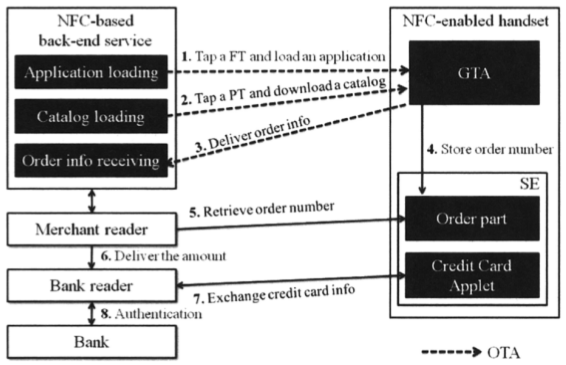
\includegraphics[width=0.5\textwidth]{creditCard.png}
        \caption{Fase de pago con \emph{modo tarjeta de crédito}.}
        \label{fig:creditCard}
      \end{center}
    \end{figure}

    \end{itemize}
  \item \textbf{Fase de envío y recogida}. En esta fase, el cliente elige
  la forma y el lugar en que recibe el producto o servicio. Para productos
  físicos elegirá el lugar al que deben llevárselo o el lugar en el que quiere
  recogerlo. Y para productos virtuales el dispositivo donde quiere
  almacenarlo.
  \item \textbf{Fase de gestión de fidelización}. El programa de fidelización
  está diseñado para incentivar al cliente a consumir de nuevo. Los cupones son
  herramientas de fidelización comunes y la tecnología \acs{NFC} hace factible
  el concepto de \emph{cupones virtuales}.
    \begin{itemize}
    \item Los clientes pueden recibir cupones tocando una etiqueta que 
    simbolice la descarga de un cupón.
    \item A través de \acs{NFC}, utilizando el modo de comunicación
    \emph{peer-to-peer}, los clientes pueden compartir sus cupones con los
    demás. Esto puede aprovecharse para desarrollar un programa de
    \emph{márketing} atractivo y eficaz.
    \end{itemize}
  \item \textbf{Fase de servicio}. Para solicitar un servicio bastará con
  tocar con el dispositivo móvil una etiqueta de tipo servicio. Las diferentes
  opciones de servicio que estén disponibles serán accesibles a través de
  otras etiquetas de servicio o mediante la selección de ese servicio en la
  pantalla del dispositivo.
  \end{itemize}
  
  Dada su generalidad, el modelo basado en el comercio móvil \acs{NMC} está 
  pensado para establecer las líneas maestras a la hora de desarrollar 
  cualquier clase de servicios móviles; entre ellos por supuesto, un sistema
  de gestión de restaurantes basado en \acs{NFC}.

    \subsection{Métodos de pago móvil a distancia}
  Hoy en día se pueden distinguir dos tipos de pagos a distancia: los que se
  producen de forma remota, como cuando se realizan compras por Internet;
  y los que se realizan dentro del mismo sitio donde se está
  comprando. El primero de ellos goza de una gran popularidad, ya que se
  considera un método fácil, cómodo y bastante seguro; y no requiere de una
  infraestructura especial para ser implementado. El segundo en cambio,
  aún no goza de la misma aceptación, debido en parte a que los 
  establecimientos no están dispuestos a invertir su dinero en adquirir una 
  infraestructura adicional para permitir este tipo de pagos, sin ver antes 
  que hacerlo les reporte algún tipo de beneficio.

  En la actualidad el pago a distancia por móvil utilizando la tecnología
  \acs{RFID} y \acs{NFC} se puede conseguir mediante uno de estos tres métodos:
  \begin{description}
  \item[SIMpass]. Es una tecnología de interfaz dual que combina la
  tradicional tarjeta \acs{SIM} y la tarjeta \acs{RFID}, en una sola tarjeta
  estándar. La interfaz de contacto cumple con la norma \acs{ISO} 7816 y la
  interfaz a distancia cumple con el estándar de la norma \acs{ISO} 14443.
  \emph{SIMpass} trabaja con una frecuencia de 13,56MHz. Como no es una
  frecuencia muy alta, es difícil minimizar el tamaño de antena. Existen dos
  maneras de implementar dicha antena. Una, de bajo coste, se lleva a cabo 
  utilizando una antena plana que consta de una bobina y que se une a la 
  del teléfono móvil. Para la otra, hay que reformar parte del hardware del 
  teléfono móvil, aunque mejora notablemente la estabilidad y fiabilidad de la
  funcionalidad \acs{RFID}.

  \item[NFC]. Como se ha visto en secciones anteriores, \acs{NFC} es una
  tecnología que combina la tecnología \acs{RFID} con las comunicaciones de
  corto alcance. En el sistema \acs{NFC} propuesto se distinguen tres partes 
  principales: el controlador, la antena y una unidad de seguridad. La unidad
  de seguridad puede correr a cargo de la tarjeta \acs{SIM} o de la tarjeta
  \acs{SD}. El problema está en que, tanto en un caso como en otro, habría que 
  integrar un módulo o chip de seguridad que no viene por defecto en estas 
  tarjetas. Esto se soluciona utilizando la tecnología \acs{NFC} mejorada 
  (\emph{eNFC}). Aunque \emph{eNFC} hace uso de la tarjeta \acs{SIM}, sólo 
  tiene que utilizar el pin C6 para poder modificar la memoria \emph{EEPROM}, 
  en vez de tener que utilizar dos pines (C4 y C8) que además interferirían a 
  la hora de realizar otras operaciones.

    \item[Programa RF-SIM]. Combinando el módulo de comunicaciones móviles y
  los micro-módulos de radio frecuencia (\emph{RF}) de la tarjeta \acs{SIM}
  normal, la tarjeta \emph{RF-SIM} consigue operar a 2,4GHz (una alta 
  frecuencia que tiene una longitud de onda corta). Esto permite que, a través
  de una antena, el módulo \emph{RF-SIM} pueda comunicarse con otros 
  dispositivos externos a distancias entre los 10 y los 500cm, a pesar de que
  dicho módulo tenga un tamaño muy reducido. \emph{RF-SIM} es un tipo de
  etiqueta activa, por lo que necesita una batería para trabajar.
  \end{description}

%%%%%%%%%%%%%%%%%%% He leído hasta aquí %%%%%%%%%%%%%%%%%%%%%%%%%%%%%%%%
%%%%%%%%%%%%%%%%%%%%%%%%%%%%%%%%%%%%%%%%%%%%%%%%%%%%%%%%%%%%%%%%%%%%%%%%

  Cada uno de estos métodos tiene sus ventajas e inconvenientes. Por ejemplo:
  \begin{itemize}
  \item Para implementar el método \emph{SIMpass} es necesario utilizar los
  pines \emph{C4} y \emph{C8}, que están reservados para la interfaz de alta
  velocidad de la tarjeta \acs{SIM}. Por lo tanto tiene un conflicto en la
  evolución futura de la tarjeta \acs{SIM}. Además, aunque la antena que
  necesita tiene un costo más asequible; la fiabilidad, el alcance y la
  velocidad de las transacciones dejan mucho que desear. Por lo que se 
  considera un método poco recomendable.
  \item La distancia de reacción es el factor más significativo de un sistema
  \acs{RFID}. Para un sistema de pago, cuanto más corta sea esta distancia
  más segura será la transacción. El programa \emph{RF-SIM} trabaja a 2.4GHz,
  lo que implica que la distancia de reacción sea demasiado larga como para ser
  segura. Los sistemas inalámbricos \texttt{Bluetooth}, \emph{Zigbee}
  \footnote{Especificación de un conjunto de protocolos de alto nivel de 
  comunicación inalámbrica para su utilización con radiodifusión digital de 
  bajo consumo, basada en el estándar IEEE 802.15.4 de redes inalámbricas de 
  área personal. Su objetivo son las aplicaciones que requieren comunicaciones 
  seguras con baja tasa de envío de datos y maximización de la vida útil de 
  sus baterías, como las aplicaciones domóticas.},
  \acs{WiFi} o \acs{UWB}\footnote{Cualquier tecnología de radio que usa un
  ancho de banda mayor de 500 MHz o del 25\% de la frecuencia central, de 
  acuerdo con la FCC (Federal Communications Commission).} usan la misma 
  frecuencia, lo que puede generar interferencias.
  \item El sistema \emph{NFC-SIM} tiene el mismo problema con los pines que
  \emph{RF-SIM} y \emph{NFC-SD} es una solución demasiado costosa.
  \item \emph{eNFC} se plantea como la solución óptima para resolver todos los
  problemas.
  \end{itemize}

  Como se decía, aunque muchos analistas e ingenieros hablan de que los 
  pagos mediante \acs{NFC} sustituirán a los pagos realizados por medios
  tradicionales, esta tecnología aún no es muy común en los teléfonos. En
  Estados Unidos, sólo dos modelos han incluido el hardware \acs{NFC}
  que soporta el pago mediante \emph{Google Wallet}\footnote{Sistema de pago 
  móvil desarrollado por \emph{Google} que permite a los usuarios guardar las 
  tarjetas de crédito, tarjetas de fidelización y tarjetas de regalo, entre 
  otras cosas. Soporta el uso de \acs{NFC}.}. En 2012 se ha anunciado
  la salida de más de 100 modelos con funcionalidad \acs{NFC} (doblando las 
  cifras del 2011). Pero sólo con la producción de más teléfonos con \acs{NFC} 
  no es suficiente. Las tiendas tienen que añadir lectores \acs{NFC} a todas
  sus cajas registradoras y los minoristas no quieren gastar dinero en esto
  hasta que la demanda no sea significativa. Por ello, mientras que esto 
  ocurre, han aparecido nuevas formas de pago que aprovechan las 
  características de otras tecnologías con las que cuentan los móviles, como 
  la lectura de códigos \acs{QR}, el acelerómetro o mediante
  \acs{SMS}~\cite{bib:noWaiting}.

    \subsection{Métodos de fidelización de clientes}
  Uno de los atractivos que puede tener el uso de la tecnología móvil \acs{NFC}
  es el de poder fidelizar a los clientes en el uso de un servicio. Para ello,
  dependiendo de las operaciones realizadas en el
  establecimiento, este puede ofrecerle productos que tal vez le interesen,
  puede proponerle descuentos por su fidelidad como cliente o puede utilizar
  el historial de todos los clientes para conocer cuáles son las tendencias
  de consumo.
  
  Uno de los últimos sistemas propuestos para sacar 
  partido a la utilización del \acs{NFC} es \emph{\textbf{WingBonus}}.

  \emph{\href{http://wingbonus.com/}{WingBonus}} es un sistema de
  gestión de promociones formado por una aplicación web y una aplicación móvil
  (disponible para sistemas \emph{Android}). Ha sido creada por el grupo de 
  investigación ISCBD (Ingeniería del Software, Conocimiento y Base de datos) 
  de la Universidad de Córdoba. Y, aunque por el momento sólo muestra 
  promociones ficticias, tiene por objetivo servir algún día de punto de 
  encuentro entre los clientes y sus marcas favoritas, a través de las 
  promociones ofertadas por estos últimos.
  
  A través de la web, los clientes pueden descargar en su móvil cupones, 
  descuentos o tarjetas de fidelización, que pueden ser utilizados a la hora 
  de realizar un pago con \acs{NFC} en los establecimientos donde tengan 
  vigencia. Es decir, si un cliente tiene un cupón de descuento para cortarse 
  el pelo en una peluquería concreta y al pagar en dicha peluquería utiliza el 
  sistema \acs{NFC}, el precio total a abonar por el corte de pelo se verá 
  decrementado por el cupón de descuento.

  El sistema permite dos tipos de usuarios: el usuario registrado y el usuario
  anónimo. Los cupones disponibles para cata tipo de usuario presentan
  características diferentes. Por ejemplo, habrá cupones en los que las
  empresas se interesen por conocer qué tipo de personas (edad, trabajo,
  estatus, etc) descargan y utilizan este tipo de cupones. Si la empresa no
  se preocupa por esta información, todo el mundo podrá descargar cupones
  como anónimo.

  Todas las ofertas que se ofrecen en la web tienen un periodo concreto de
  disponibilidad dentro del cual el cliente puede hacerse con dicha oferta
  (figura \ref{fig:wingBonusP}). Además, las ofertas tienen un tiempo acotado
  de validez que delimita el periodo en el que puede aplicarse dicha oferta.

  \begin{figure}[!h]
    \begin{center}
      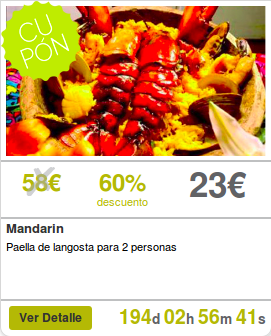
\includegraphics[width=0.5\textwidth]{wingBonusP.png}
      \caption{Ejemplo de cupón ofrecido en la web de \emph{WingBonus}.}
      \label{fig:wingBonusP}
    \end{center}
  \end{figure}

  Los cupones de descuentos tienen la particularidad de que pueden compartirse
  con otros usuarios \acs{NFC} mediante una comunicación \emph{peer-to-peer}.

  Para las empresas asociadas, \emph{WingBonus} ofrece grandes ventajas: 
  reducción de costos, eliminación del papel, poder llegar a más clientes,
  eliminación de las falsificaciones, análisis de mercado, estudio de
  tendencias, fidelización de clientes, etc.~\cite{bib:wingBonus}.

  \section{Aplicaciones comerciales}
  A continuación, se muestran varios ejemplos de cómo distintos programas
  comerciales implementan las funcionalidades típicas de los gestores de
  restaurantes. Después, se expondrán algunas aplicaciones que permiten
  realizar pedidos desde el sitio sin necesidad de tener que avisar al
  camarero.

    \subsection{Gestión de operaciones típicas de un restaurante}
    En la actualidad existe una innumerable oferta de aplicaciones que ayudan
    a gestionar las labores típicas de un restaurante, como pueden ser:
    gestionar pedidos, generar facturas o realizar la función de caja 
    registradora.

    \begin{itemize}
    \item Para \textbf{gestionar pedidos} las aplicaciones suelen contar con 
    un panel de productos en el que se van seleccionando: cantidad, producto y 
    mesa a la que va destinado (figuras \ref{fig:productsPanel} y
    \ref{fig:productsPanel2}). Normalmente la iteración consiste en: primero,
    seleccionar una mesa; después, seleccionar la cantidad; y por último,
    seleccionar el producto.

    \begin{figure}[!h]
      \begin{center}
        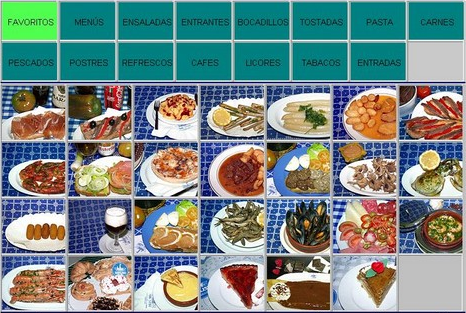
\includegraphics[width=0.8\textwidth]{productsPanel.png}
        \caption{Panel de productos del programa
        \emph{FrontRest}~\cite{bib:frontRest}.}
        \label{fig:productsPanel}
      \end{center}
    \end{figure}

    \begin{figure}[!h]
      \begin{center}
        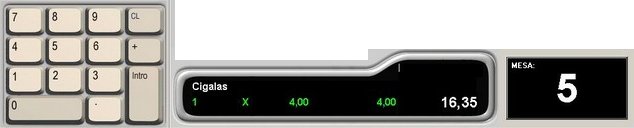
\includegraphics[width=0.8\textwidth]{productsPanel2.png}
        \caption{Panel de selección de cantidad del programa
        \emph{FrontRest}~\cite{bib:frontRest}.}
        \label{fig:productsPanel2}
      \end{center}
    \end{figure}

    Una vez terminada la iteración anterior, el pedido queda reflejado en la
    lista de productos asignados a esa mesa (figura \ref{fig:productsList}).

    \begin{figure}[!h]
      \begin{center}
        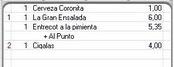
\includegraphics[width=0.5\textwidth]{productsList.png}
        \caption{Lista de pedidos para la mesa 5.
        \emph{FrontRest}~\cite{bib:frontRest}.}
        \label{fig:productsList}
      \end{center}
    \end{figure}

    \item A la hora de \textbf{facturar una mesa}, este tipo de aplicaciones 
    suelen presentar un resumen con los datos de la mesa a facturar, la lista 
    de pedidos realizados, el importe parcial de cada uno de ellos, el importe
    subtotal y el importe total con impuestos incluidos (figura
    \ref{fig:bill}).

    \begin{figure}[!h]
      \begin{center}
        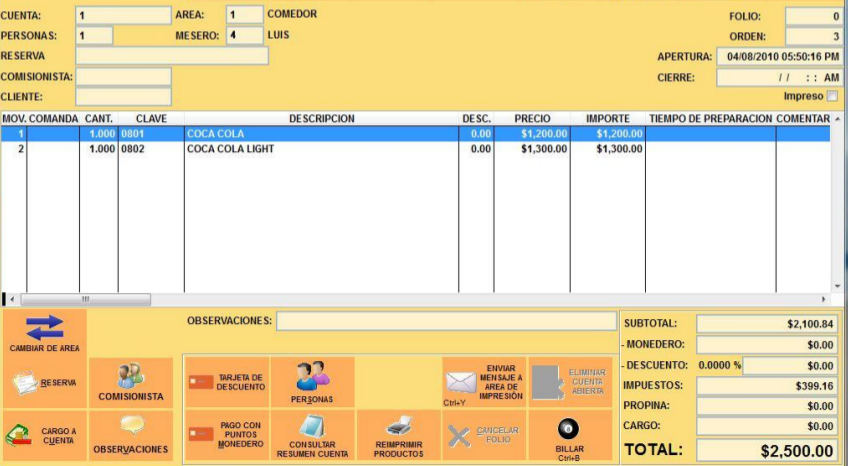
\includegraphics[width=1\textwidth]{bill.png}
        \caption{Resumen de facturación de una mesa en el programa
        \emph{Soft Restaurant}~\cite{bib:softRestaurant}.}
        \label{fig:bill}
      \end{center}
    \end{figure}

    Con estos datos, el camarero conoce en tiempo real cuál es la lista de
    productos de una mesa y cuál es el importe total que los comensales deben
    abonar en concepto de los productos consumidos.

    \item Los \textbf{productos} con los que estos programas trabajan, deben 
    ser editados por los responsables del restaurante. Entre los atributos que
    estos poseen están: código, nombre, categoría o precio (figura
    \ref{fig:editProduct}).

    \begin{figure}[!h]
      \begin{center}
        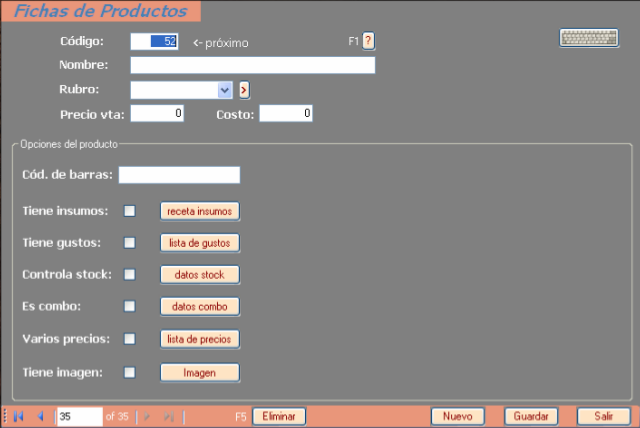
\includegraphics[width=0.8\textwidth]{editProduct.png}
        \caption{Editor de productos del programa
        \emph{SaleYa}~\cite{bib:saleYa}.}
        \label{fig:editProduct}
      \end{center}
    \end{figure}
    \end{itemize}

    Estas son las funcionalidades básicas que todo software de 
    gestión de restaurante debe tener. Pero, aparte de estas, son muchas otras 
    las funcionalidades que pueden ayudar a mejorar la gestión de un 
    restaurante.

    \begin{itemize}
    \item Es muy común en casi todos los programas de gestión de restaurantes
    buscar una \textbf{representación aproximada de las partes que forman el
    restaurante}. En un principio, lo que más interesa es representar las 
    mesas del restaurante, aunque hay aplicaciones que representan también
    la barra, las mesas del salón, las mesas de la terraza y otros objetos
    (figura \ref{fig:tables}).

    \begin{figure}[!h]
      \begin{center}
        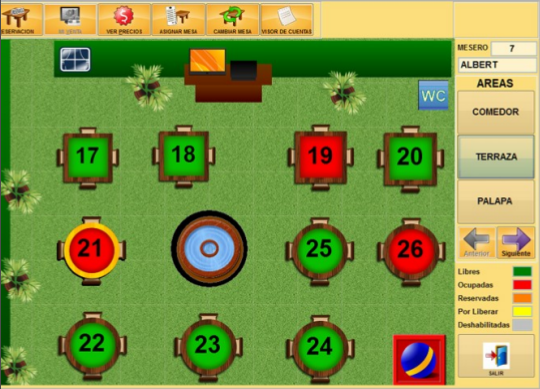
\includegraphics[width=0.8\textwidth]{tables.png}
        \caption{Mapa de un restaurante de la aplicación
        \emph{Soft Restaurant}~\cite{bib:softRestaurant}.}
        \label{fig:tables}
      \end{center}
    \end{figure}

    Estos mapas ayudan a los camareros a reconocer el estado en el que se
    encuentran las mesas (ocupadas, libres, reservadas, deshabilitadas, etc.).
    Los símbolos del mapa ayudan a ubicar dónde se encuentran los objetos
    reales a los que representan y su color representa el estado en el que
    se encuentran.

    \item Aplicaciones como \emph{Soft Restaurant}~\cite{bib:softRestaurant} o 
    \emph{SaleYa}~\cite{bib:saleYa} tienen una funcionalidad que permite 
    \textbf{describir las recetas} de los productos contemplados en la carta. 
    Es decir, permite listar los ingredientes (con sus cantidades) utilizados 
    en la elaboración de cada plato (figura \ref{fig:ingredients}). Esto 
    facilita la gestión del \emph{stock} de dichos ingredientes.

    \begin{figure}[!h]
      \begin{center}
        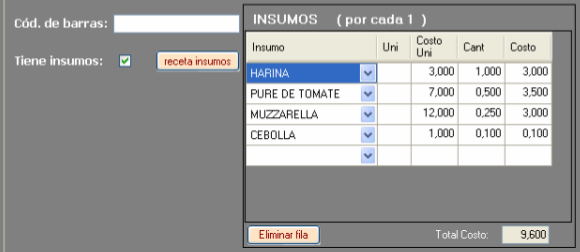
\includegraphics[width=0.8\textwidth]{ingredients.png}
        \caption{Ingredientes para la elaboración de una \emph{pizza de 
        mozzarella}. \emph{SaleYa}~\cite{bib:saleYa}.}
        \label{fig:ingredients}
      \end{center}
    \end{figure}

    Esta funcionalidad ayuda a los cocineros y a sus ayudantes a conocer
    mejor cuáles son los ingredientes necesarios para la elaboración de 
    un plato y les ayuda a gestionar de una manera más eficiente el
    \emph{stock} de los ingredientes, según las necesidades que la 
    elaboración cada plato demande.

    \item Una funcionalidad que puede ser muy útil a la hora de gestionar
    los pedidos es incorporar un terminal en la cocina, para que los cocineros
    informen del \textbf{estado de preparación de las comandas} (figura
    \ref{fig:kitchen}).

    \begin{figure}[!h]
      \begin{center}
        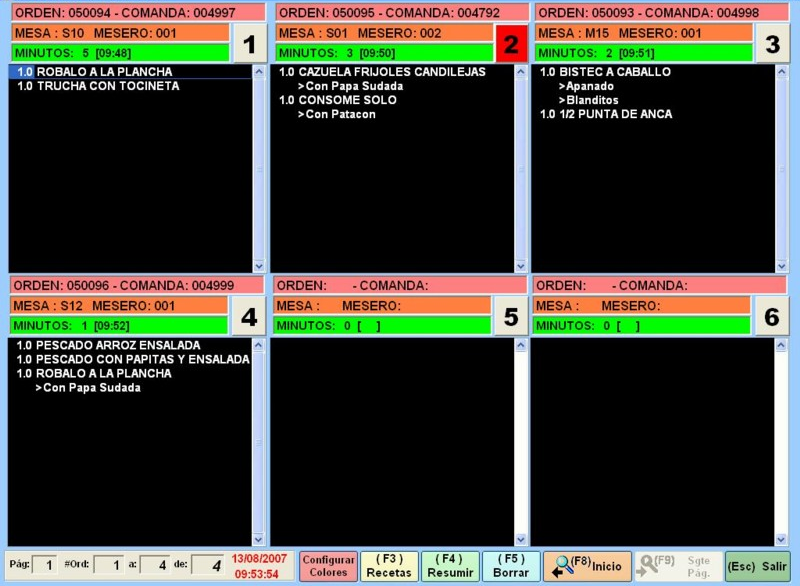
\includegraphics[width=0.8\textwidth]{kitchen.png}
        \caption{Monitor de comandas de la aplicación
        \emph{RestBar}~\cite{bib:restBar}.}
        \label{fig:kitchen}
      \end{center}
    \end{figure}
    
    La aplicación muestra qué camarero ha solicitado el plato, la hora en que
    lo solicitó y los minutos que han pasado desde que lo hizo. Cuando los
    productos están listos para servir, los cocineros informan a los
    camareros, cambiando el estado del pedido a través de la aplicación.

    \item Si el restaurante tiene entre sus servicios el \textbf{reparto a
    domicilio}, no está demás que la aplicación cuente con una funcionalidad
    en la que quede constancia de los pedidos a domicilio que tiene pendientes
    (figura \ref{fig:deliveries}):

    \begin{figure}[!h]
      \begin{center}
        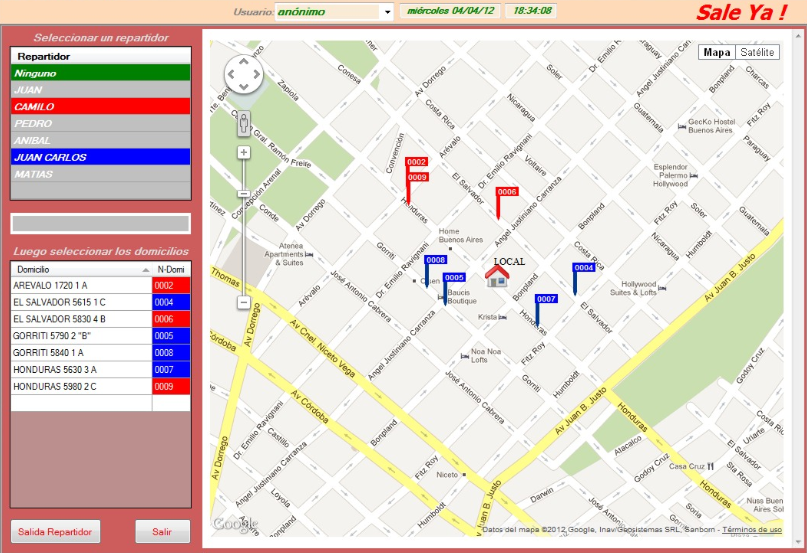
\includegraphics[width=0.8\textwidth]{deliveries.png}
        \caption{Módulo que gestiona los repartos a domicilio.
        \emph{SaleYa}~\cite{bib:saleYa}.}
        \label{fig:deliveries}
      \end{center}
    \end{figure}

    La aplicación registra cuáles son los pedidos pendientes, qué repartidor
    se encargará de atenderlos y dónde están los puntos de entrega.
    \end{itemize}

    El abanico de programas de gestión de restaurantes es muy diverso. A la
    hora de adquirir uno u otro conviene determinar bien qué necesidades de
    información se deben satisfacer, de tal forma que no se eche en falta 
    ninguna funcionalidad y que no se tengan funcionalidades incompatibles
    con el modelo de negocio que se posee.

    \subsection{Gestión de pedidos a través de dispositivos móviles}
    Las soluciones vistas en el apartado anterior van encaminadas a
    facilitar las tareas propias de los camareros y cocineros del restaurante,
    pero en ninguna de ellas se tiene en cuenta al cliente. Si el cliente es
    capaz de realizar pedidos sin necesidad de avisar a un camarero, este
    quedará liberado para realizar otras tareas.

    A continuación, se presentan dos soluciones comerciales que buscan
    satisfacer este objetivo:

    \begin{itemize}
    \item \textbf{vMenu}. Es un sistema ideado por la empresa \emph{Vloo} que
    trata de reinventar la carta tradicional adentrándose en el mundo
    interactivo actual, a través de las pantallas táctiles. Los clientes
    disponen de un dispositivo (\emph{iPad}, tablet o pantalla) en la que
    pueden ver los platos disponibles y realizar los pedidos (figura
    \ref{fig:starters}).

    \begin{figure}[!h]
      \begin{center}
        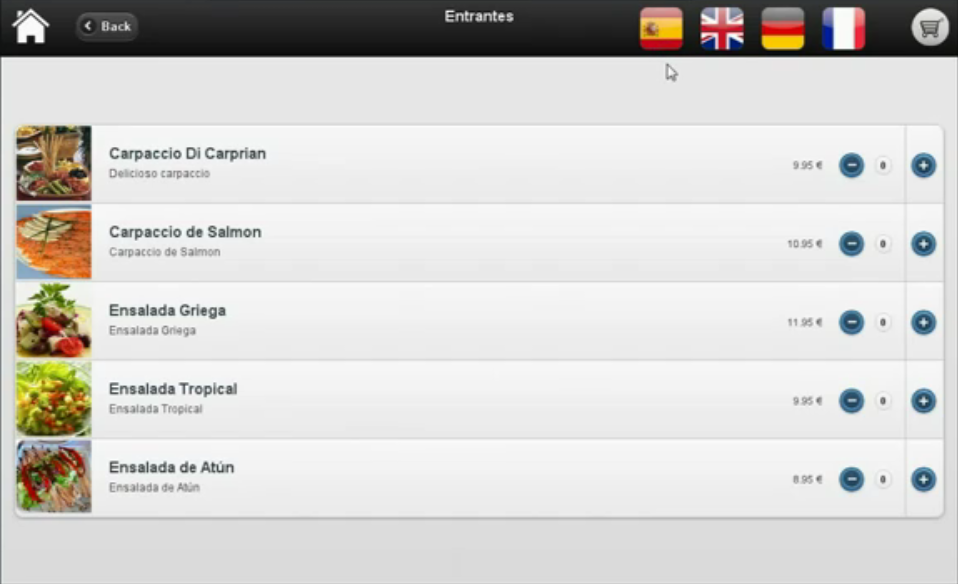
\includegraphics[width=0.8\textwidth]{starters.png}
        \caption{Lista de productos \emph{entrantes}.}
        \label{fig:starters}
      \end{center}
    \end{figure}

    Los productos aparecen distribuidos por categorías y son actualizados
    de manera instantánea. Además, los alimentos son mostrados de una forma
    más atractiva: con fotos, ingredientes, recetas, calorías, preparación y 
    otros datos de interés; y siempre en el idioma del comensal (figura
    \ref{fig:meat}).

    \begin{figure}[!h]
      \begin{center}
        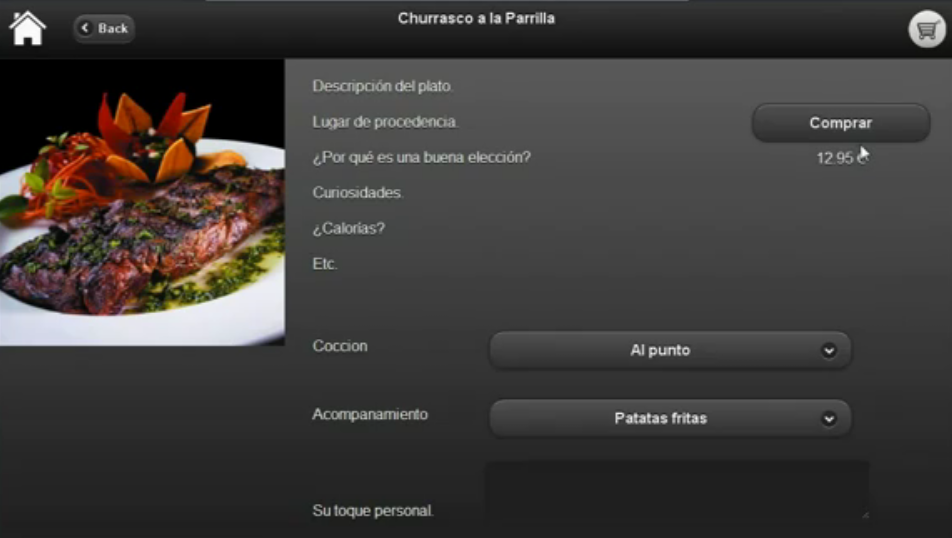
\includegraphics[width=0.8\textwidth]{meat.png}
        \caption{Información asociada al \emph{churrasco a la parrilla}.}
        \label{fig:meat}
      \end{center}
    \end{figure}
    
    \emph{vMenu} reduce los tiempos de espera porque el cliente no necesita
    al camarero para conocer los productos, las recomendaciones o las ofertas
    disponibles; ni para realizar el pedido (figura \ref{fig:order}) o
    solicitar la cuenta; y en caso de necesitarlo, dispone de una opción para
    llamarlo desde el terminal.

    \begin{figure}[!h]
      \begin{center}
        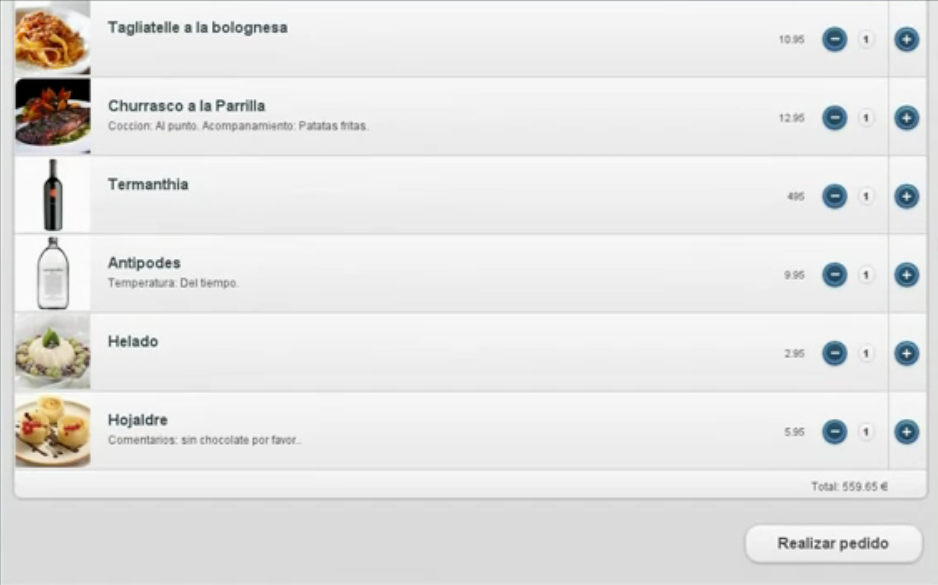
\includegraphics[width=0.8\textwidth]{order.png}
        \caption{Lista de productos elegidos para un pedido.}
        \label{fig:order}
      \end{center}
    \end{figure}

    Por último, a parte de esta función de recogida de pedidos, \emph{vMenu} 
    dispone de todo un sistema integral que permite gestionar las operaciones
    básicas de un restaurante~\cite{bib:vMenu}.

    \item \textbf{Brand Table}. \emph{S-Digital}, una \emph{start-up} de la
    Universidad de Sidney, ofrece este prototipo conceptual de mesa de
    restaurante en torno a la cual se distribuyen varios menús electrónicos con
    los que se puede interactuar utilizando un dispositivo móvil con \acs{NFC}
    (figura \ref{fig:brandTable}), de forma que los comensales que se reúnan a 
    su alrededor puedan seleccionar su comida favorita y pagarla
    \emph{in situ} (utilizando \emph{Google Wallet} o \emph{Paypal Mobile}), 
    sin necesidad de tener que esperar a ningún camarero que les tome nota del 
    pedido (figura \ref{fig:brandTableDemo}).

    \begin{figure}[!h]
      \begin{center}
        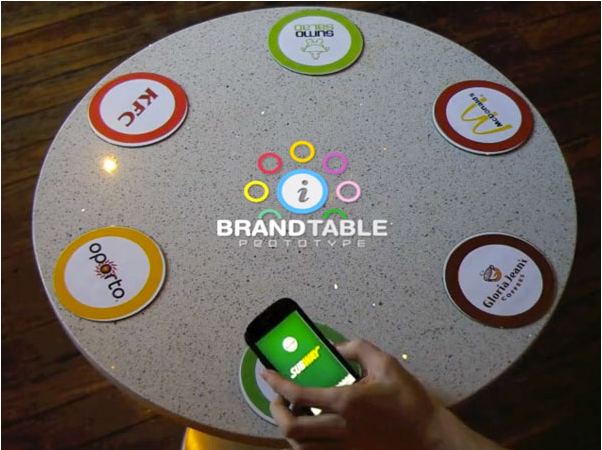
\includegraphics[width=0.6\textwidth]{brandTable.png}
        \caption{Prototipo conceptual de la mesa \emph{Brand Table}.}
        \label{fig:brandTable}
      \end{center}
    \end{figure}

    \begin{figure}[!h]
      \begin{center}
        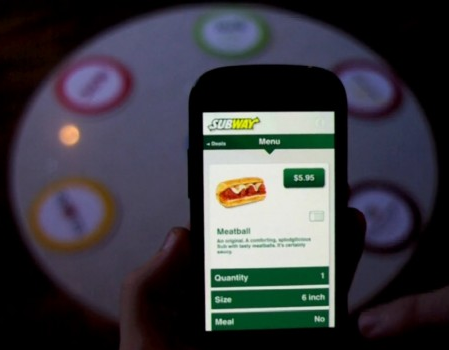
\includegraphics[width=0.6\textwidth]{brandTableDemo.png}
        \caption{Selección de uno de los productos del restaurante
        \emph{Subway}.}
        \label{fig:brandTableDemo}
      \end{center}
    \end{figure}

    Cuando el pedido está preparado, el cliente se levanta y va a recogerlo.
    
    Este sistema está pensado para restaurantes de comida rápida y elimina
    completamente la labor del camarero~\cite{bib:brandTable}.
    \end{itemize}


% Local Variables:
%   coding: utf-8
%   mode: latex
%   mode: flyspell
%   ispell-local-dictionary: "castellano8"
% End:
